\section{Heritability of house sparrow traits}
We now investigate the results of applying our method to the house sparrow dataset. As mentioned, estimating the heritability of phenotypic traits can be seen as a special case of relative variable importance. The findings we present here are direct calculations obtained by our method. We present the samples of relative variable importance obtained of the variance component that captures additive genetic variance, and use the results from \citet{Silva2017} and \citet{Muff2019Genetic} to compare with. In \Cref{tab:summary_heritability} the mean of sampled heritability along with confidence intervals is presented, as well as the corresponding measures from the comparable studies.

\begin{table}[ht]
  \centering
  \begin{tabular}{lccccccc}
  \toprule
   & \multicolumn{2}{c}{\citet{Silva2017}} & \multicolumn{2}{c}{\citet{Muff2019Genetic}} & \multicolumn{2}{c}{BVI} \\ 
   \cmidrule(lr){2-3} \cmidrule(lr){4-5} \cmidrule(lr){6-7}
   & Estimate & CI & Estimate & CI & Mean & CI \\ 
  \midrule
  $h^2_{\text{mass}}$    & 0.300 & [0.2314, 0.3686] & 0.2875 & [0.2188, 0.3707] & 0.2841 & [0.2324 0.3442] \\
  $h^2_{\text{wing}}$    & 0.388 & [0.3525, 0.4605] & 0.3438 & [0.2939, 0.4085] & 0.3543 & [0.3208 0.3906] \\
  $h^2_{\text{tarsus}}$  & 0.415 & [0.3327, 0.4973] & - & - & 0.4016 & [0.3305 0.4690] \\ 
  \bottomrule
  \end{tabular}
  \caption{Heritability estimates and confidence interval from \citet{Silva2017}, posterior means of additive genetic variance divided by the posterior means of total phenotypic variance in \citet{Muff2019Genetic} with corresponding confidence interval and the mean and confidence interval of the heritability samples obtained from the BVI method for the phenotypic traits; body mass, wing length and tarsus length.}
  \label{tab:summary_heritability}
\end{table}

For the sampled heritability of body mass (\Cref{fig:heritability_mass}), we have a mean of $0.2841$ and a distribution which seems slightly skewed to the left. The mean and mode seem to be approximately the same. 

The samples of wing length heritability form a smooth bell curve with a mean of $0.3543$ (\Cref{fig:heritability_wing}). Also here the mean and mode seem to be roughly the same, but the distribution is more symmetric than for body mass.

The heritability samples of tarsus length (\Cref{fig:heritability_tarsus}) has a mean of $0.4016$ and a distribution that has three distinct peaks. The center peak is the highest, and the peaks on each side seem to be of equal height. We suspect that this pattern is a result of how INLA performs the sampling of the LMM. The mean and mode are approximately the same.



\begin{figure}[H]
    \centering
      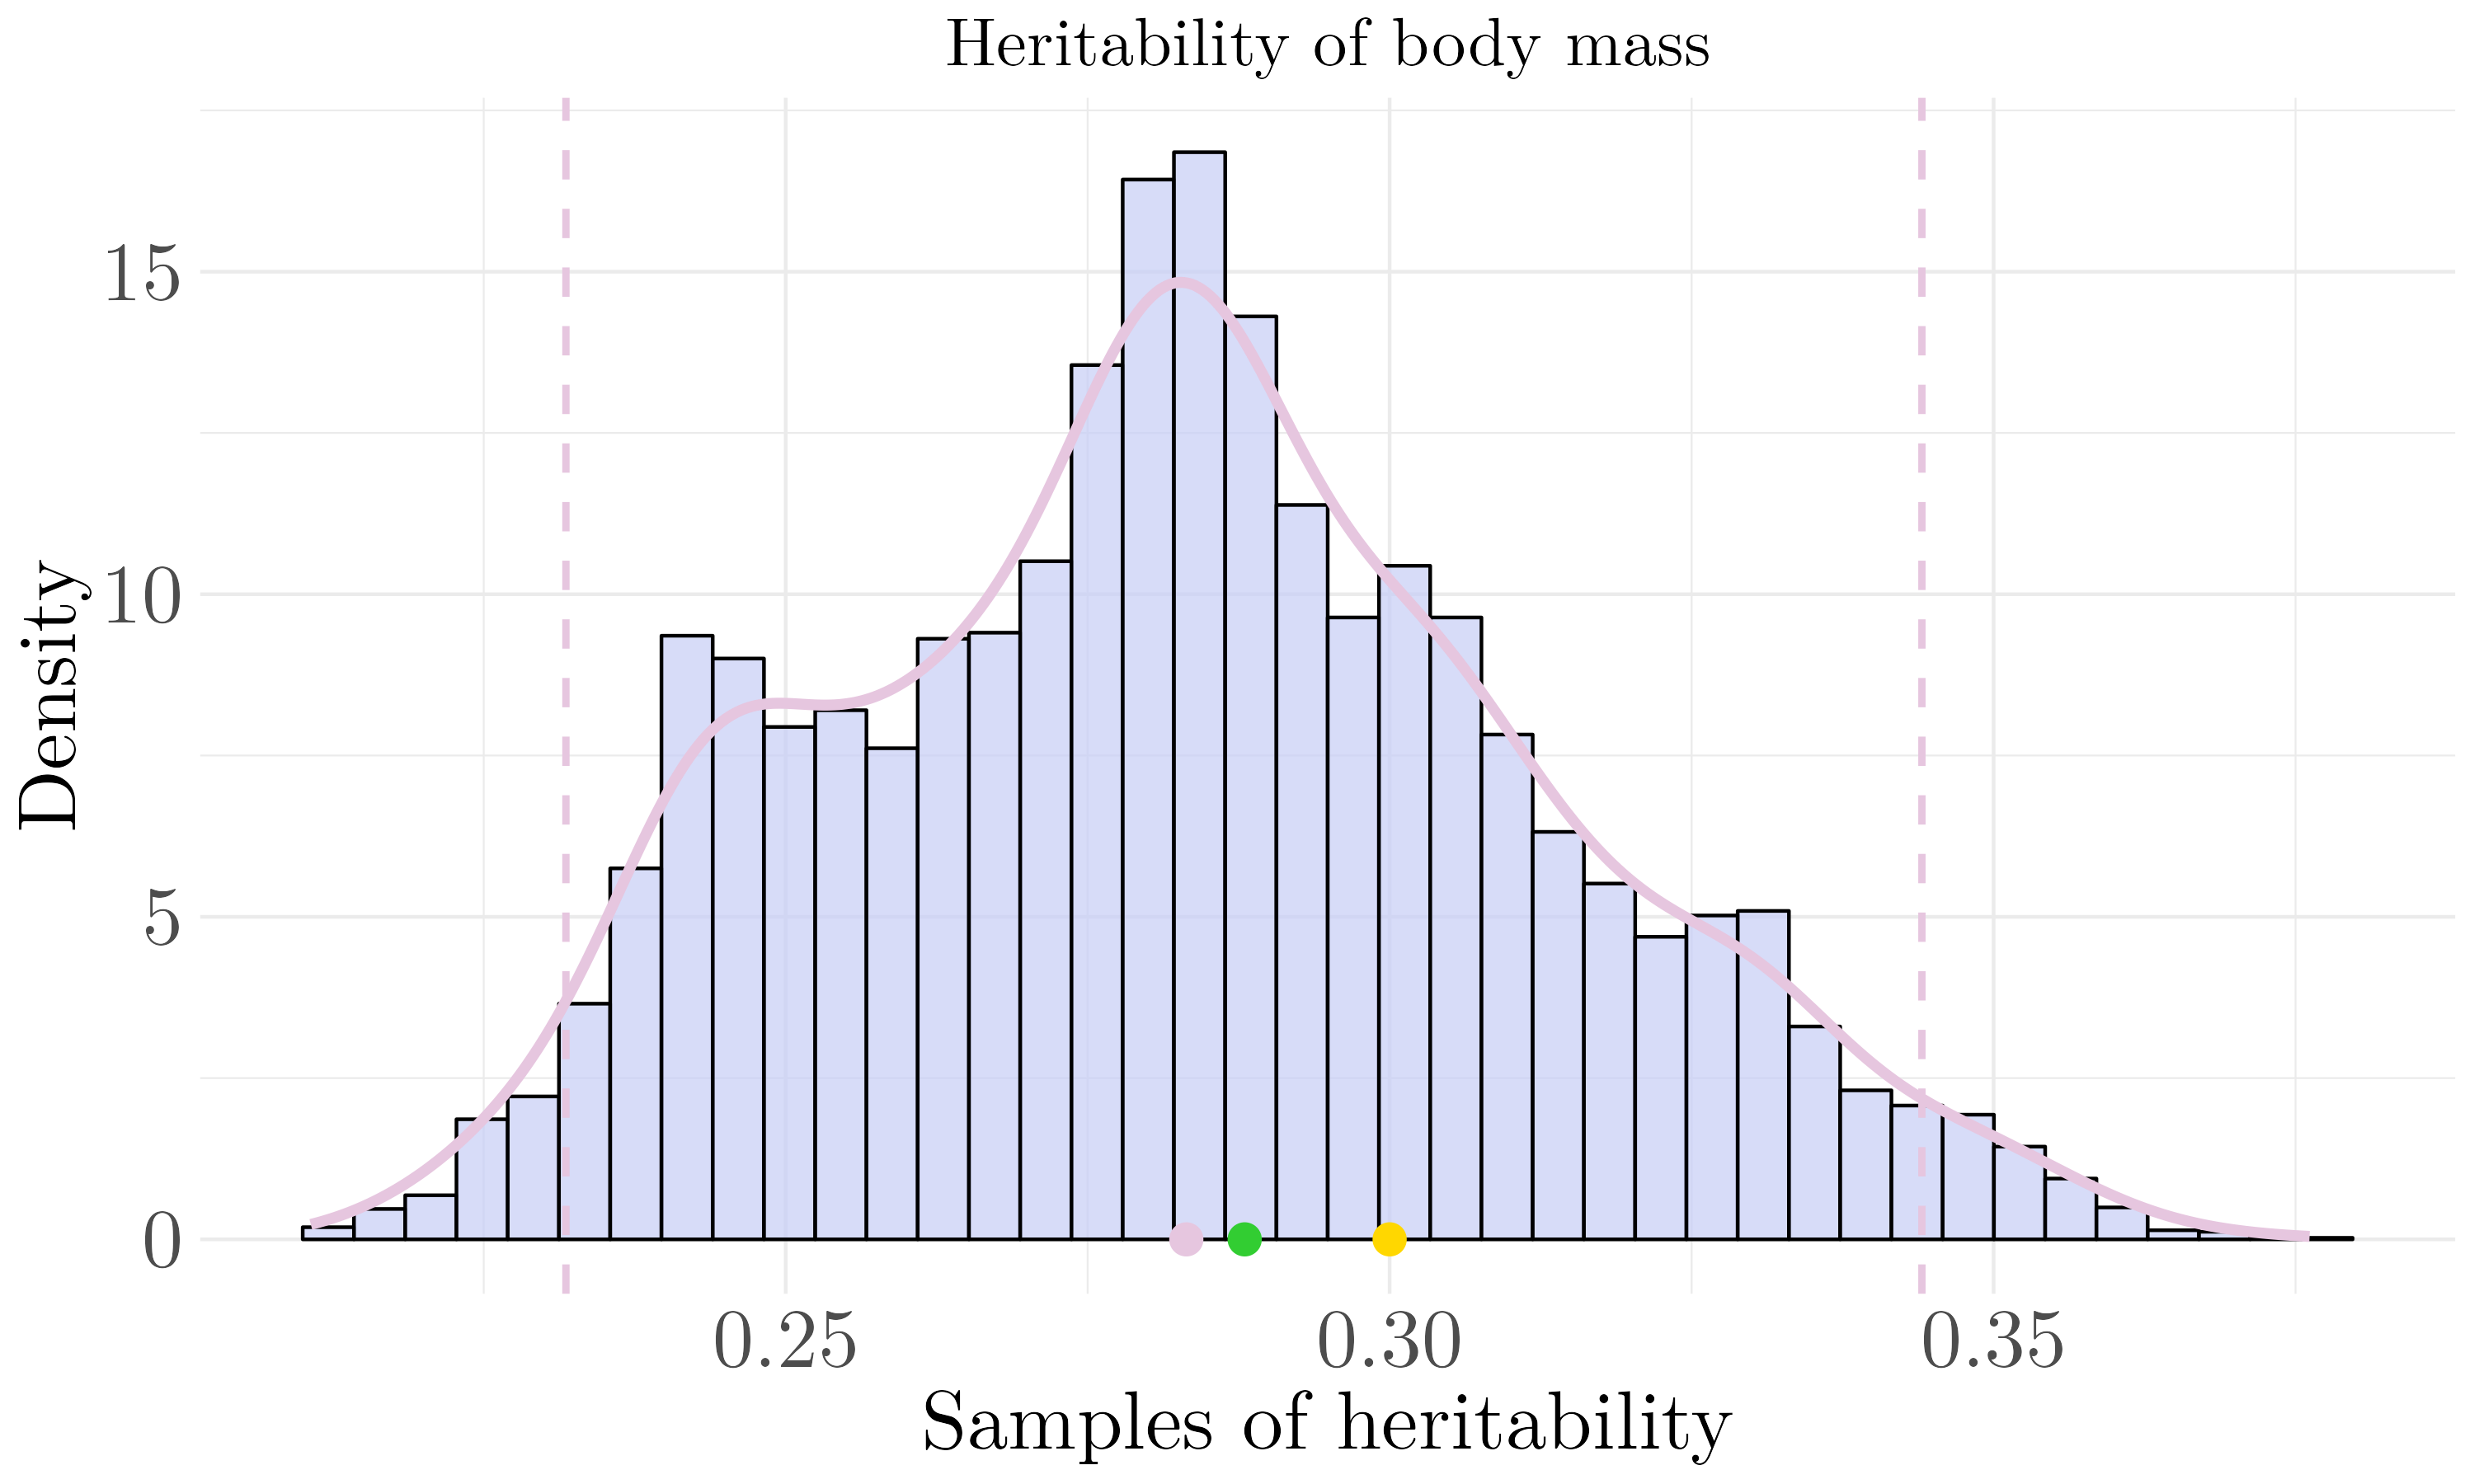
\includegraphics[width=0.7\linewidth]{Figures/House sparrow study/Heritability_mass.png}
      \caption{Heritability of body mass}
      \label{fig:heritability_mass}
  \end{figure}
  \begin{figure}[H]%\ContinuedFloat
    \centering
    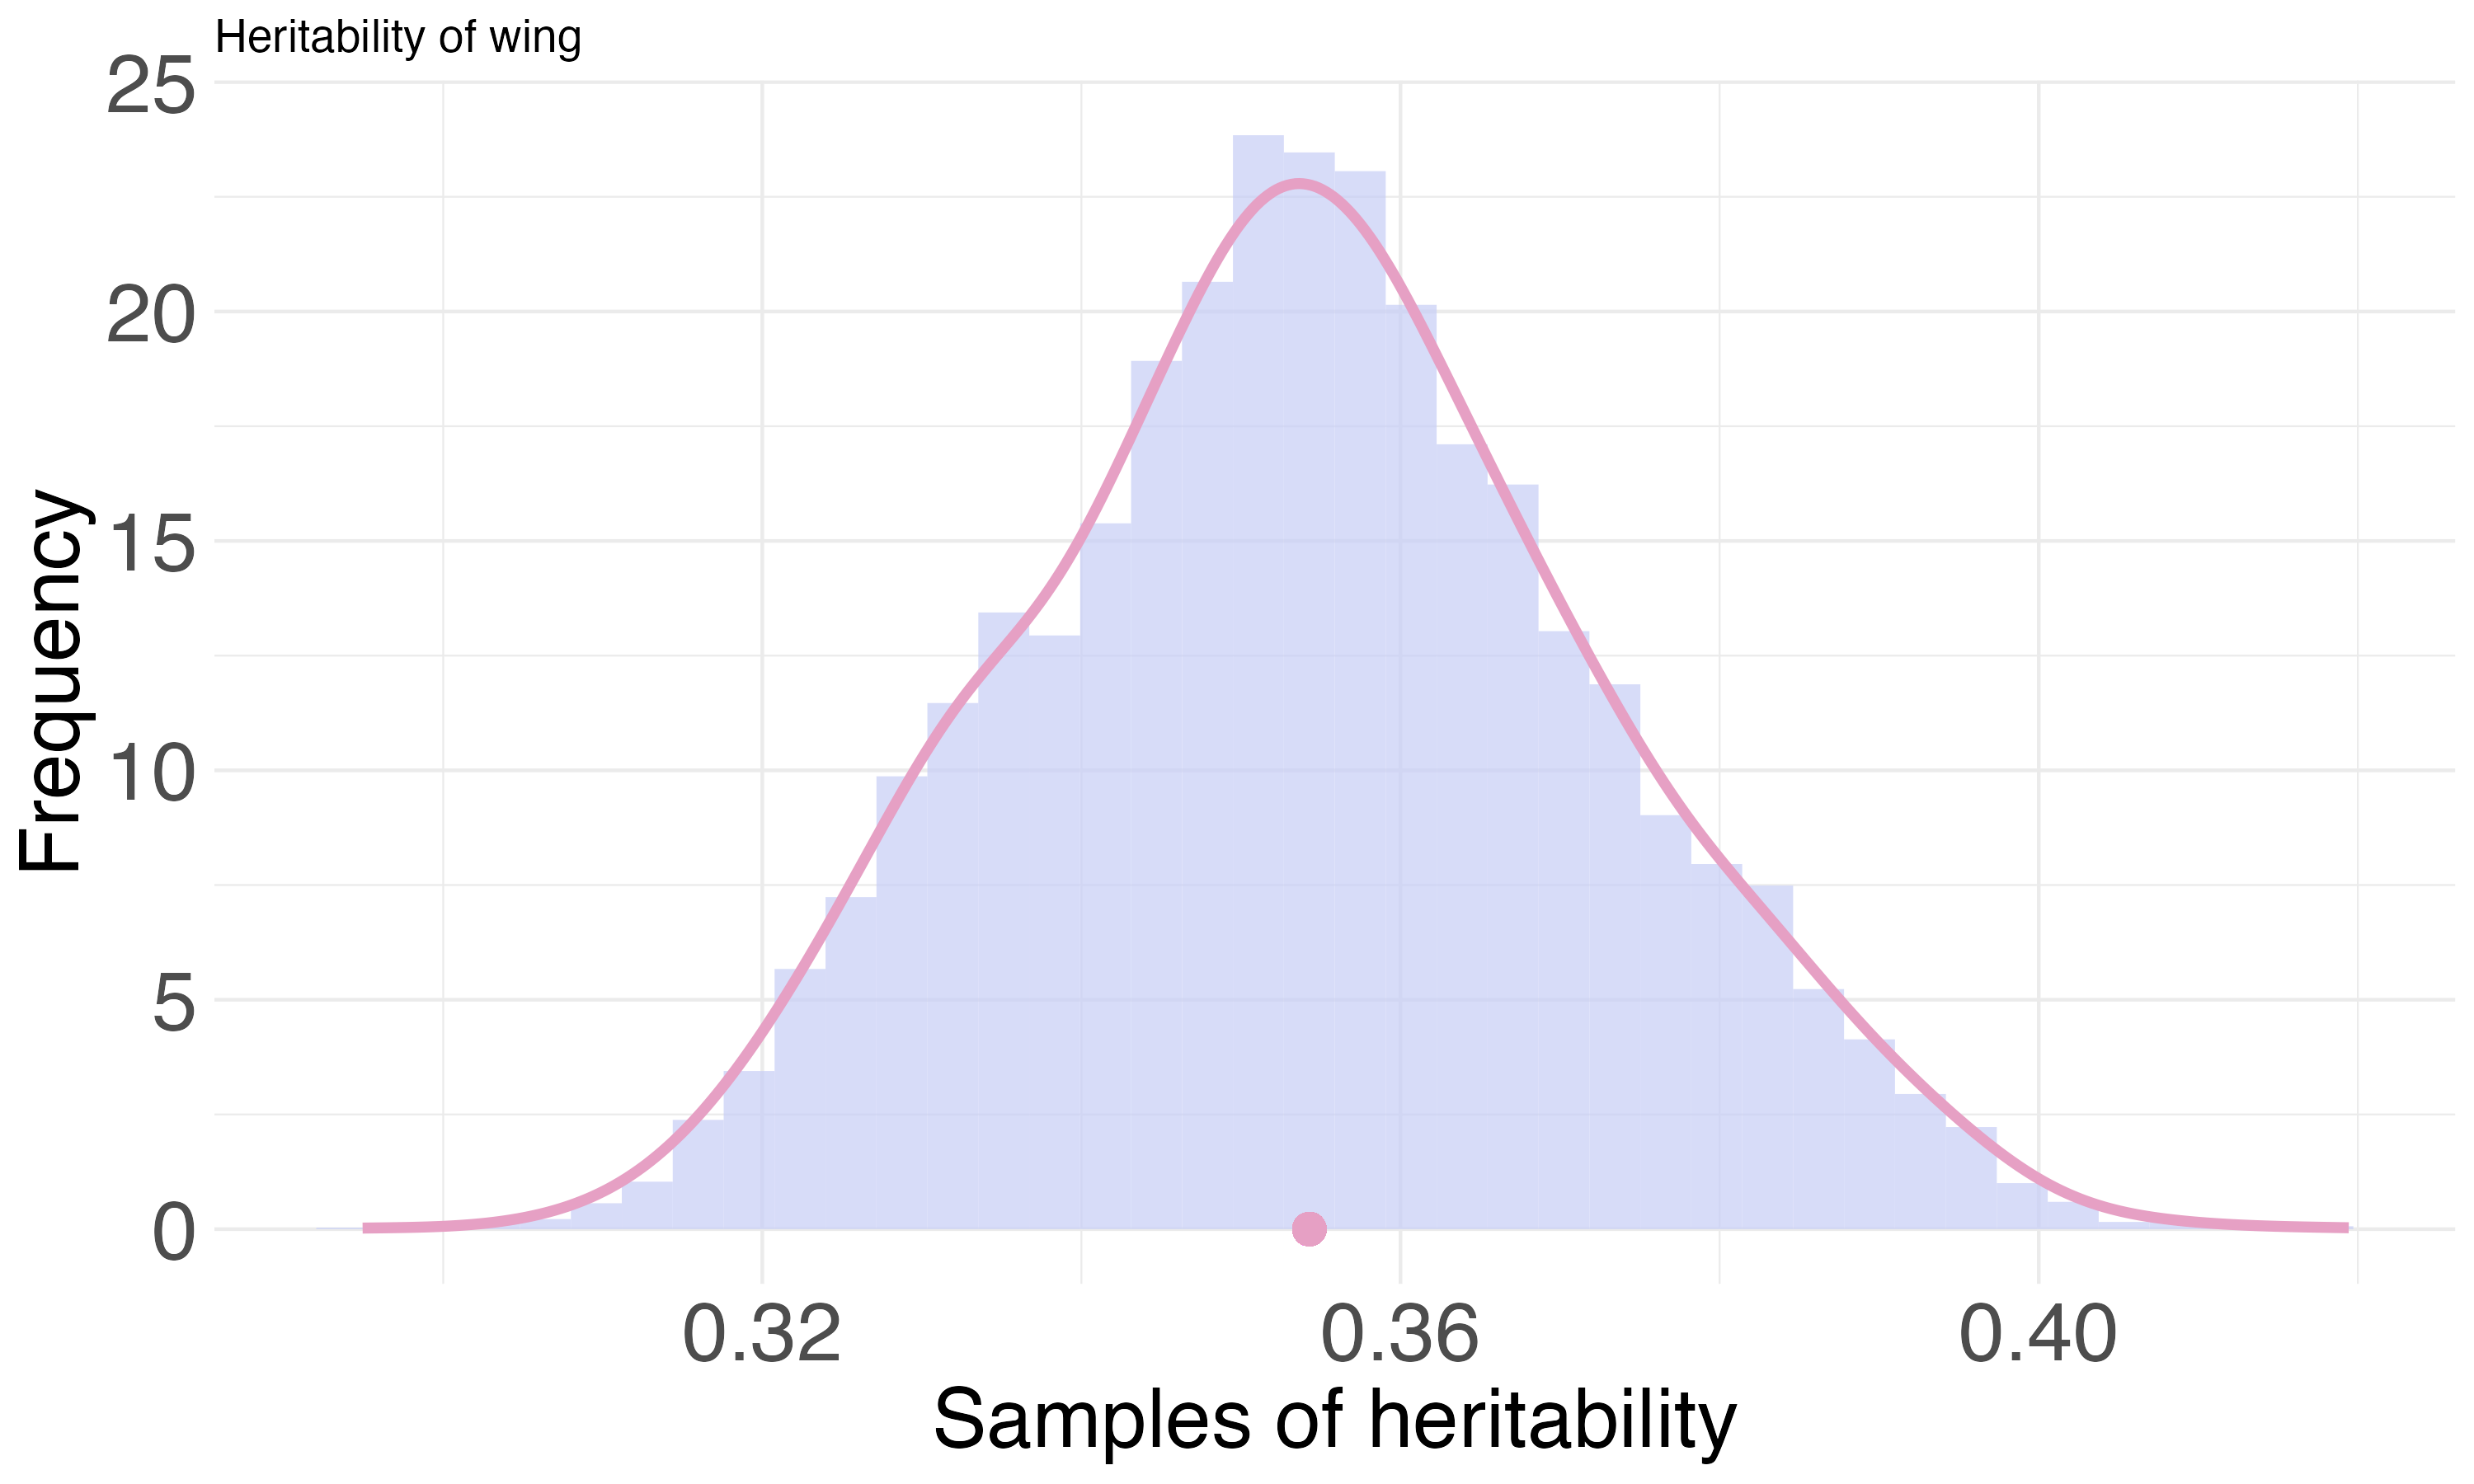
\includegraphics[width=0.7\linewidth]{Figures/House sparrow study/Heritability_wing.png}
    \caption{Heritability of wing length}
    \label{fig:heritability_wing}
  \end{figure}
  \begin{figure}[H]%\ContinuedFloat
    \centering
    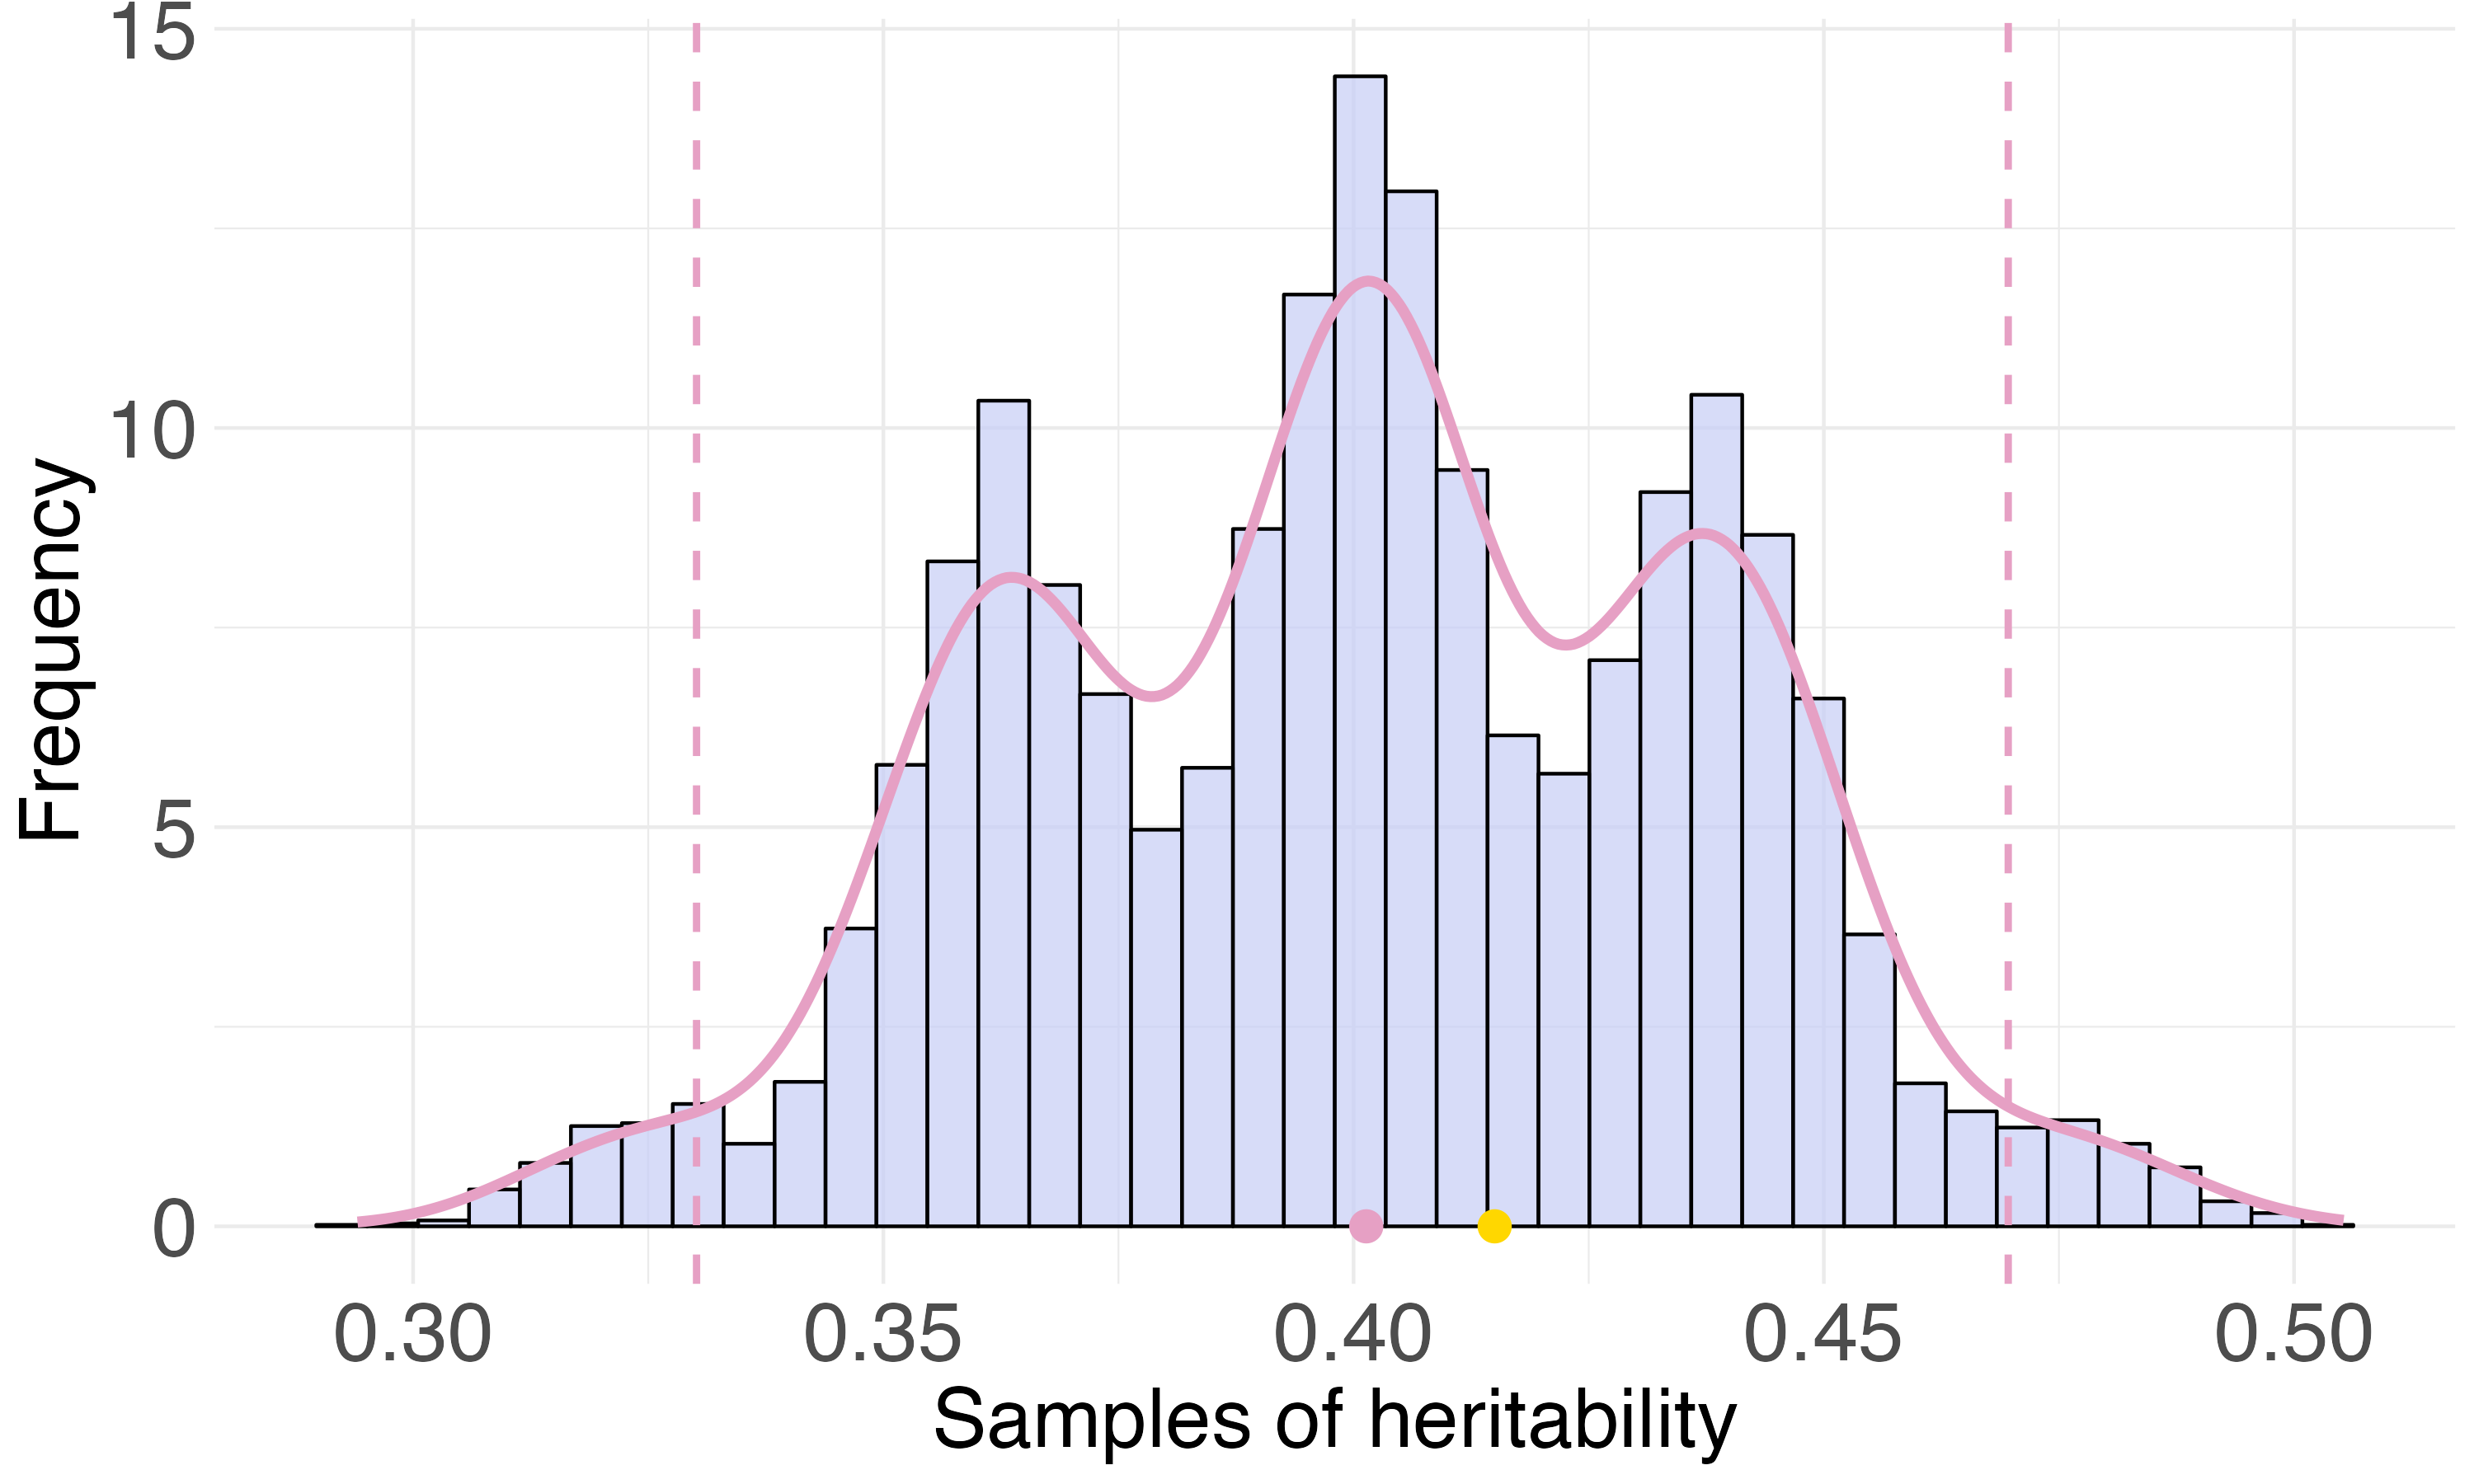
\includegraphics[width=0.7\linewidth]{Figures/House sparrow study/Heritability_tarsus.png}
    \caption{Heritability of tarsus length}
    \label{fig:heritability_tarsus}
  \end{figure}

\section{Comparison with \texttt{rptR} package}

% \begin{figure}[H]
%     \centering
%       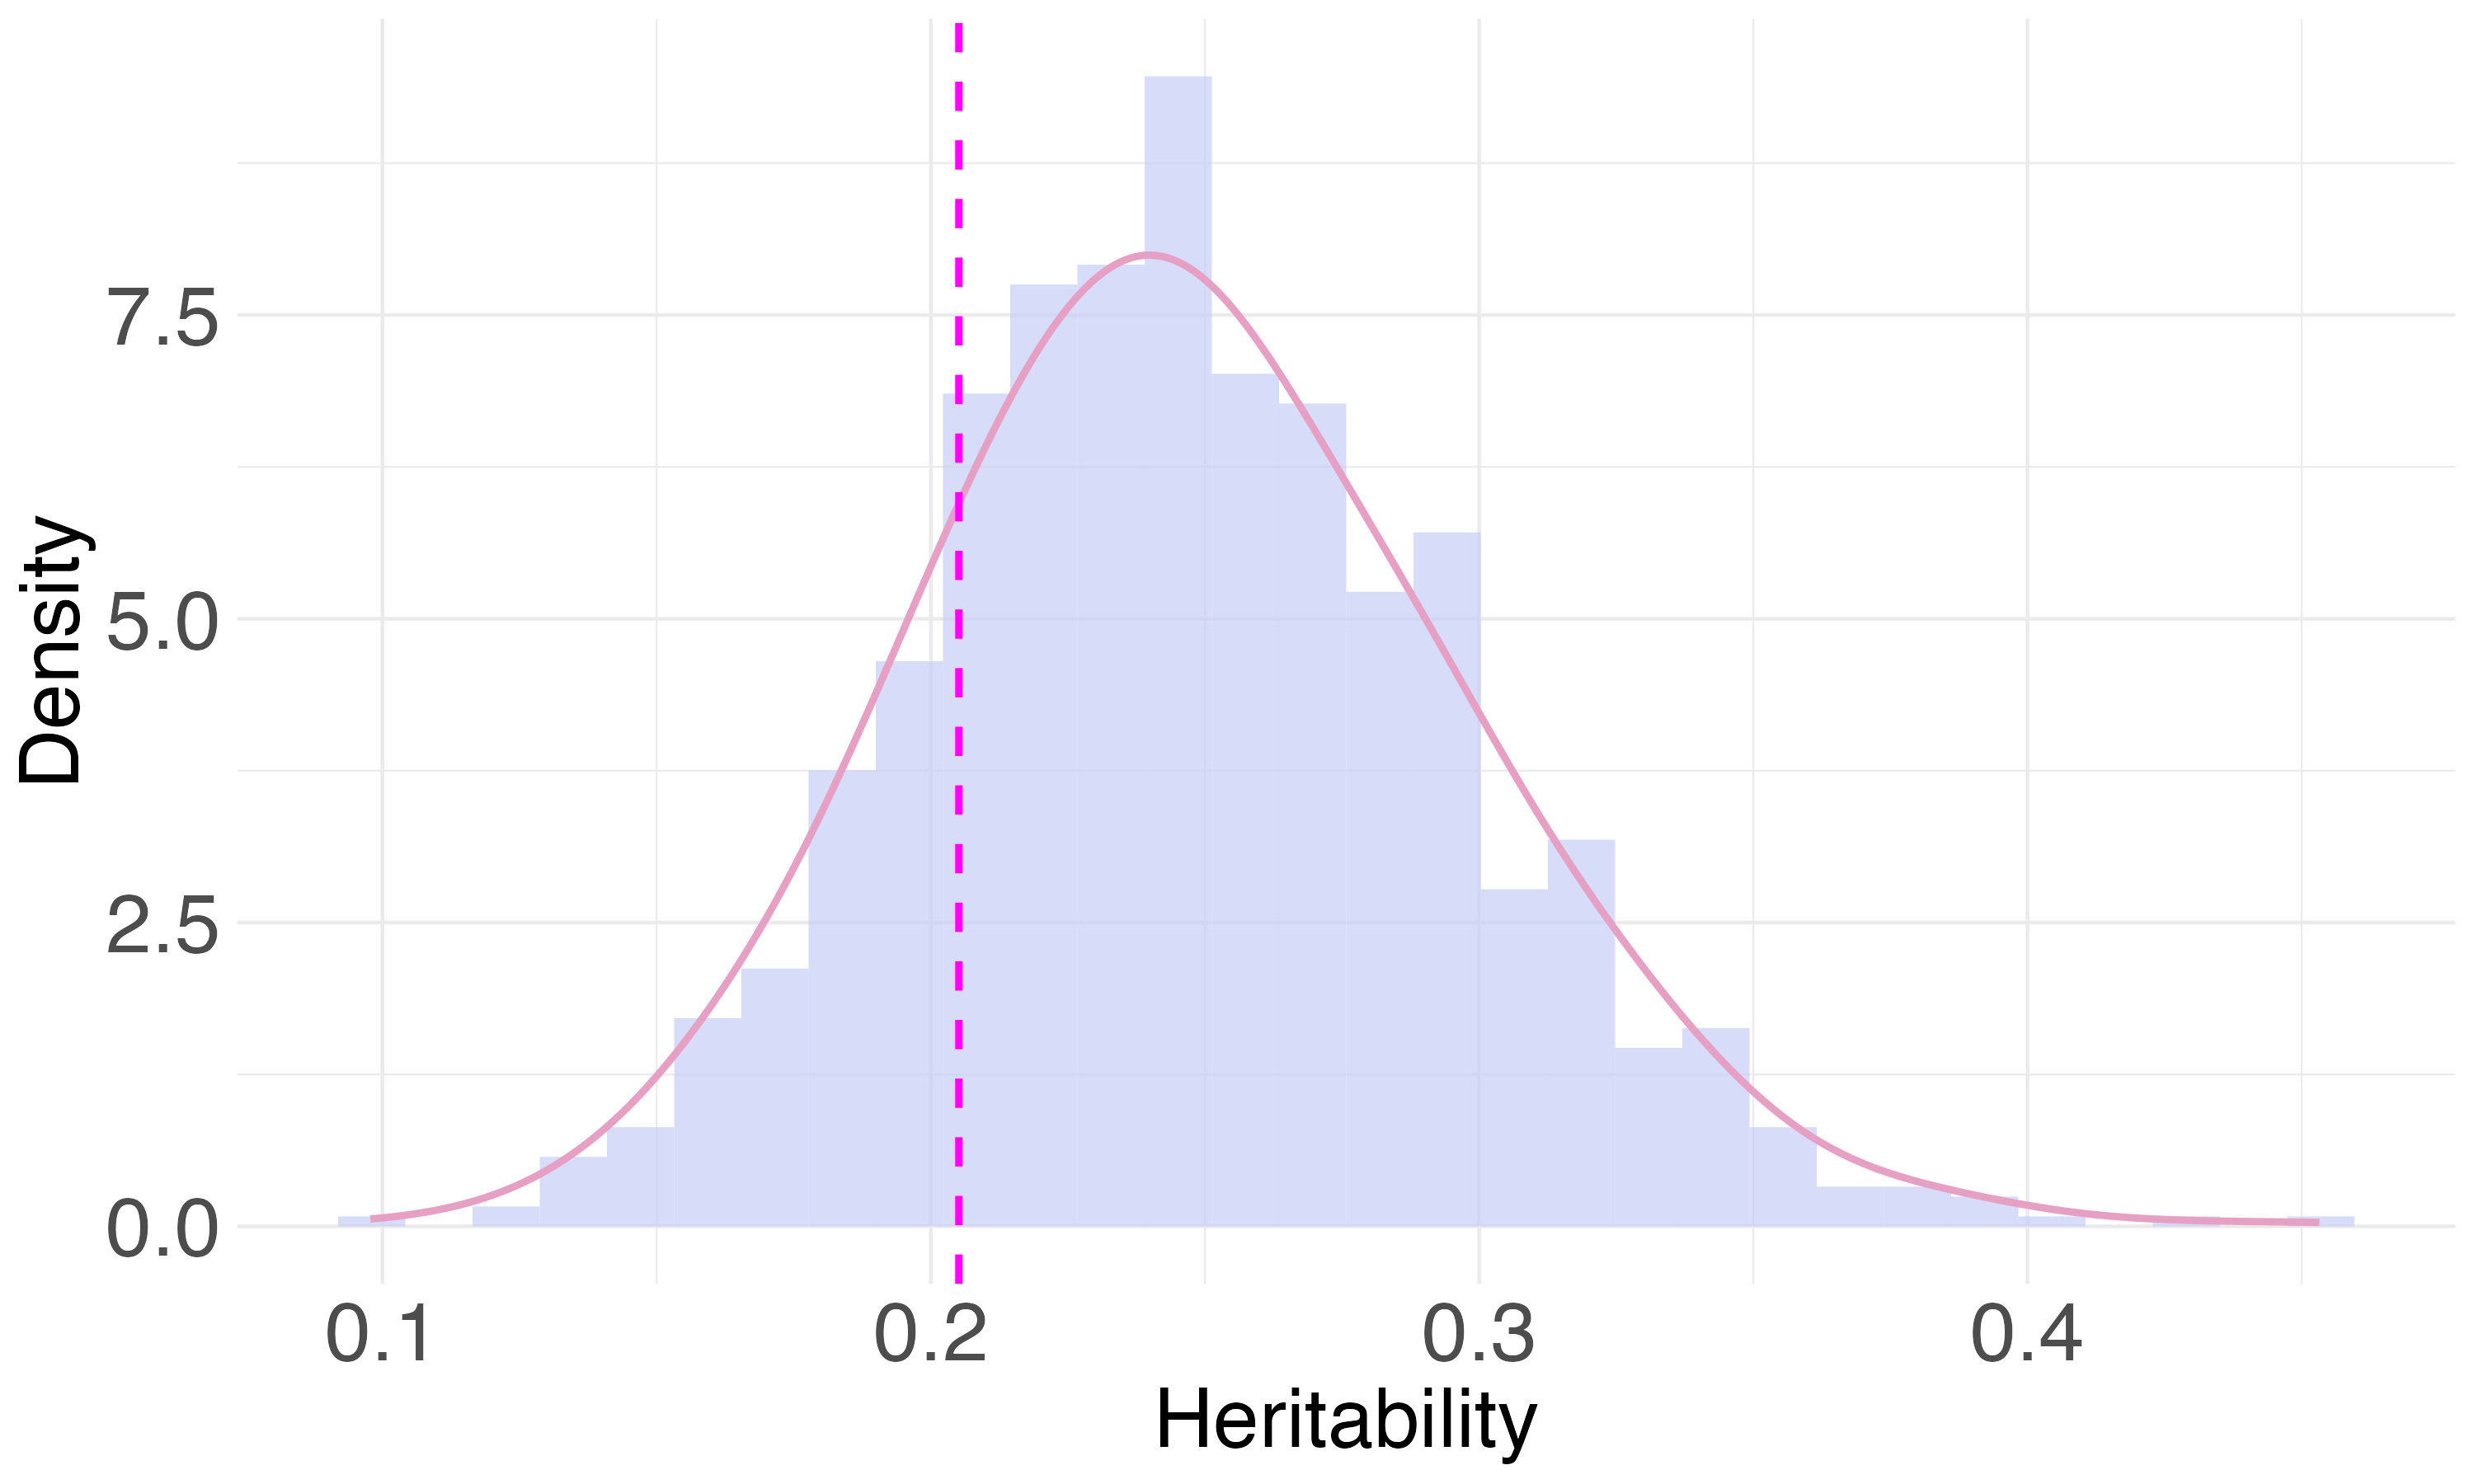
\includegraphics[width=0.7\linewidth]{Figures/Stoffel Comparison/Heritability_colour_binomial.png}
%       \caption{Heritability of colour of male beetles from Stoffel}
%       \label{fig:heritability_colour_binomial}
%   \end{figure}
%   \begin{figure}[H]\ContinuedFloat
%     \centering
%     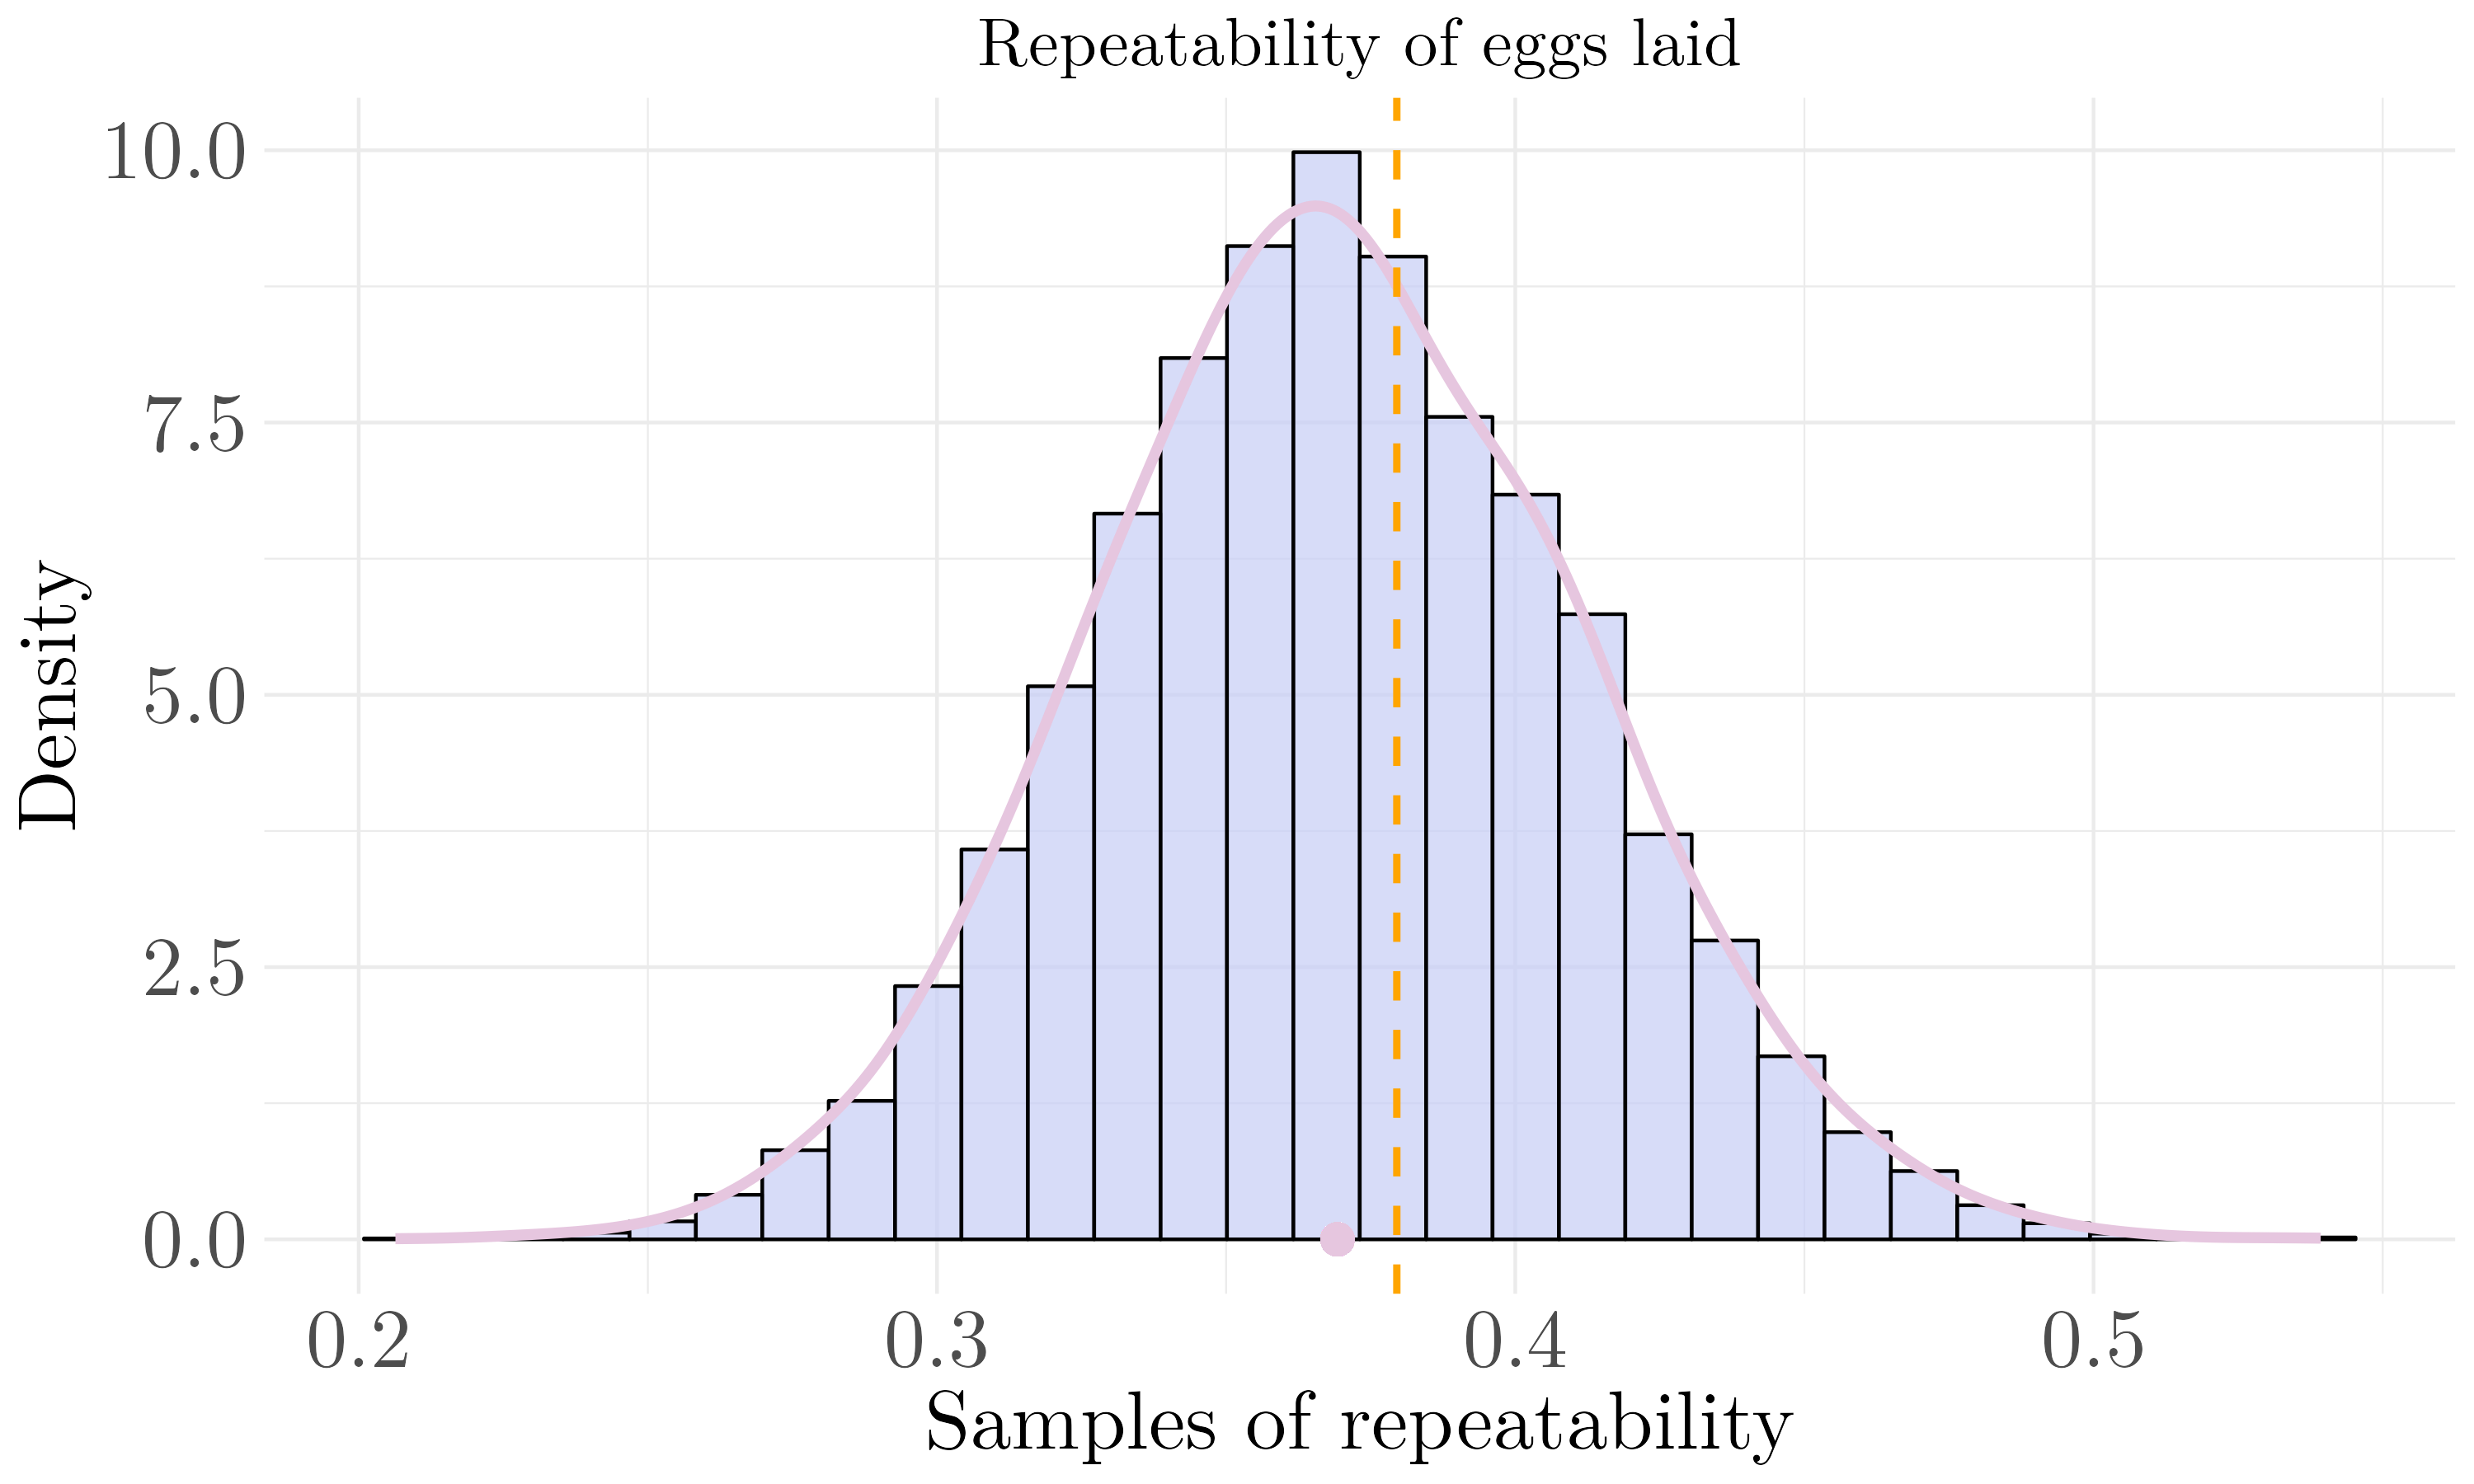
\includegraphics[width=0.7\linewidth]{Figures/Stoffel Comparison/Heritability_egg_poisson.png}
%     \caption{Heritability of eggs laid by female beetles from Stoffel}
%       \label{fig:heritability_egg_poisson}
%   \end{figure}


\begin{figure}[!ht]
  \centering
  % First row
  \subfloat{
    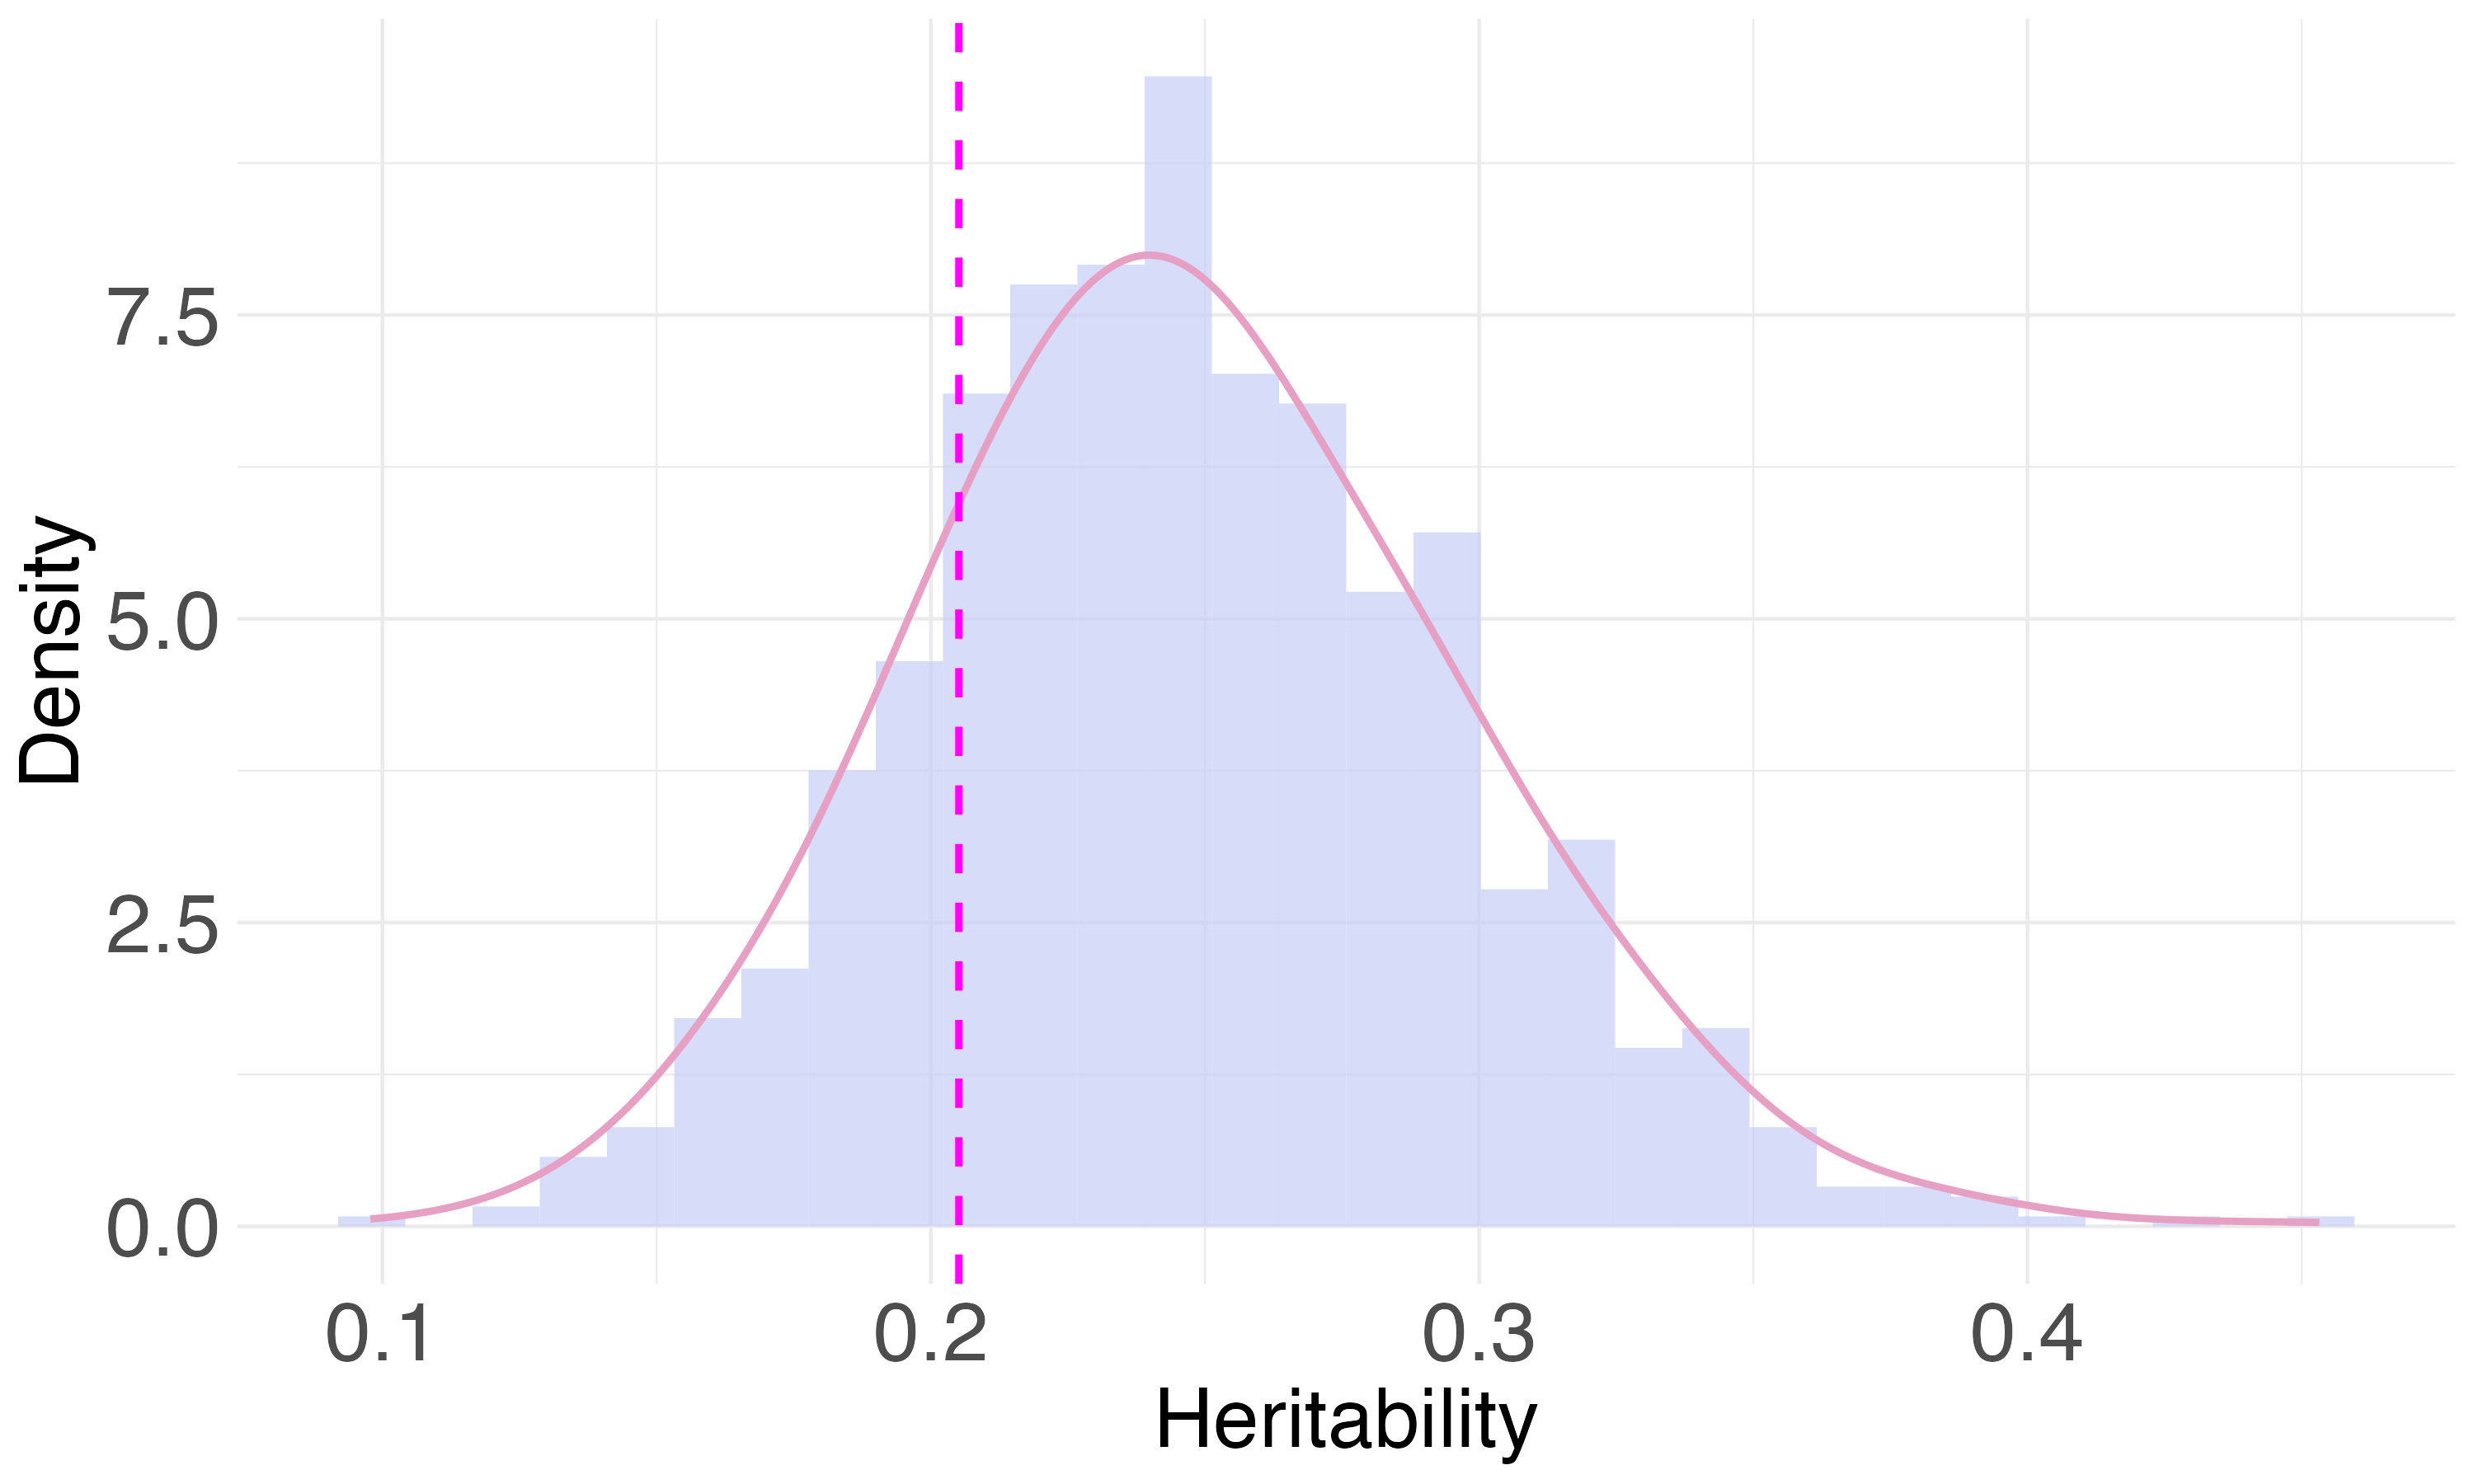
\includegraphics[width=0.6\linewidth]{Figures/Stoffel Comparison/Heritability_colour_binomial.png}
    \label{fig:heritability_colour_binomial}
  }
  \caption{Heritability of color of male beetles from BVI method (top) and Stoffel (bottom)}
\end{figure}

\begin{figure}[!ht]
  \centering
  % First row
  \subfloat{
    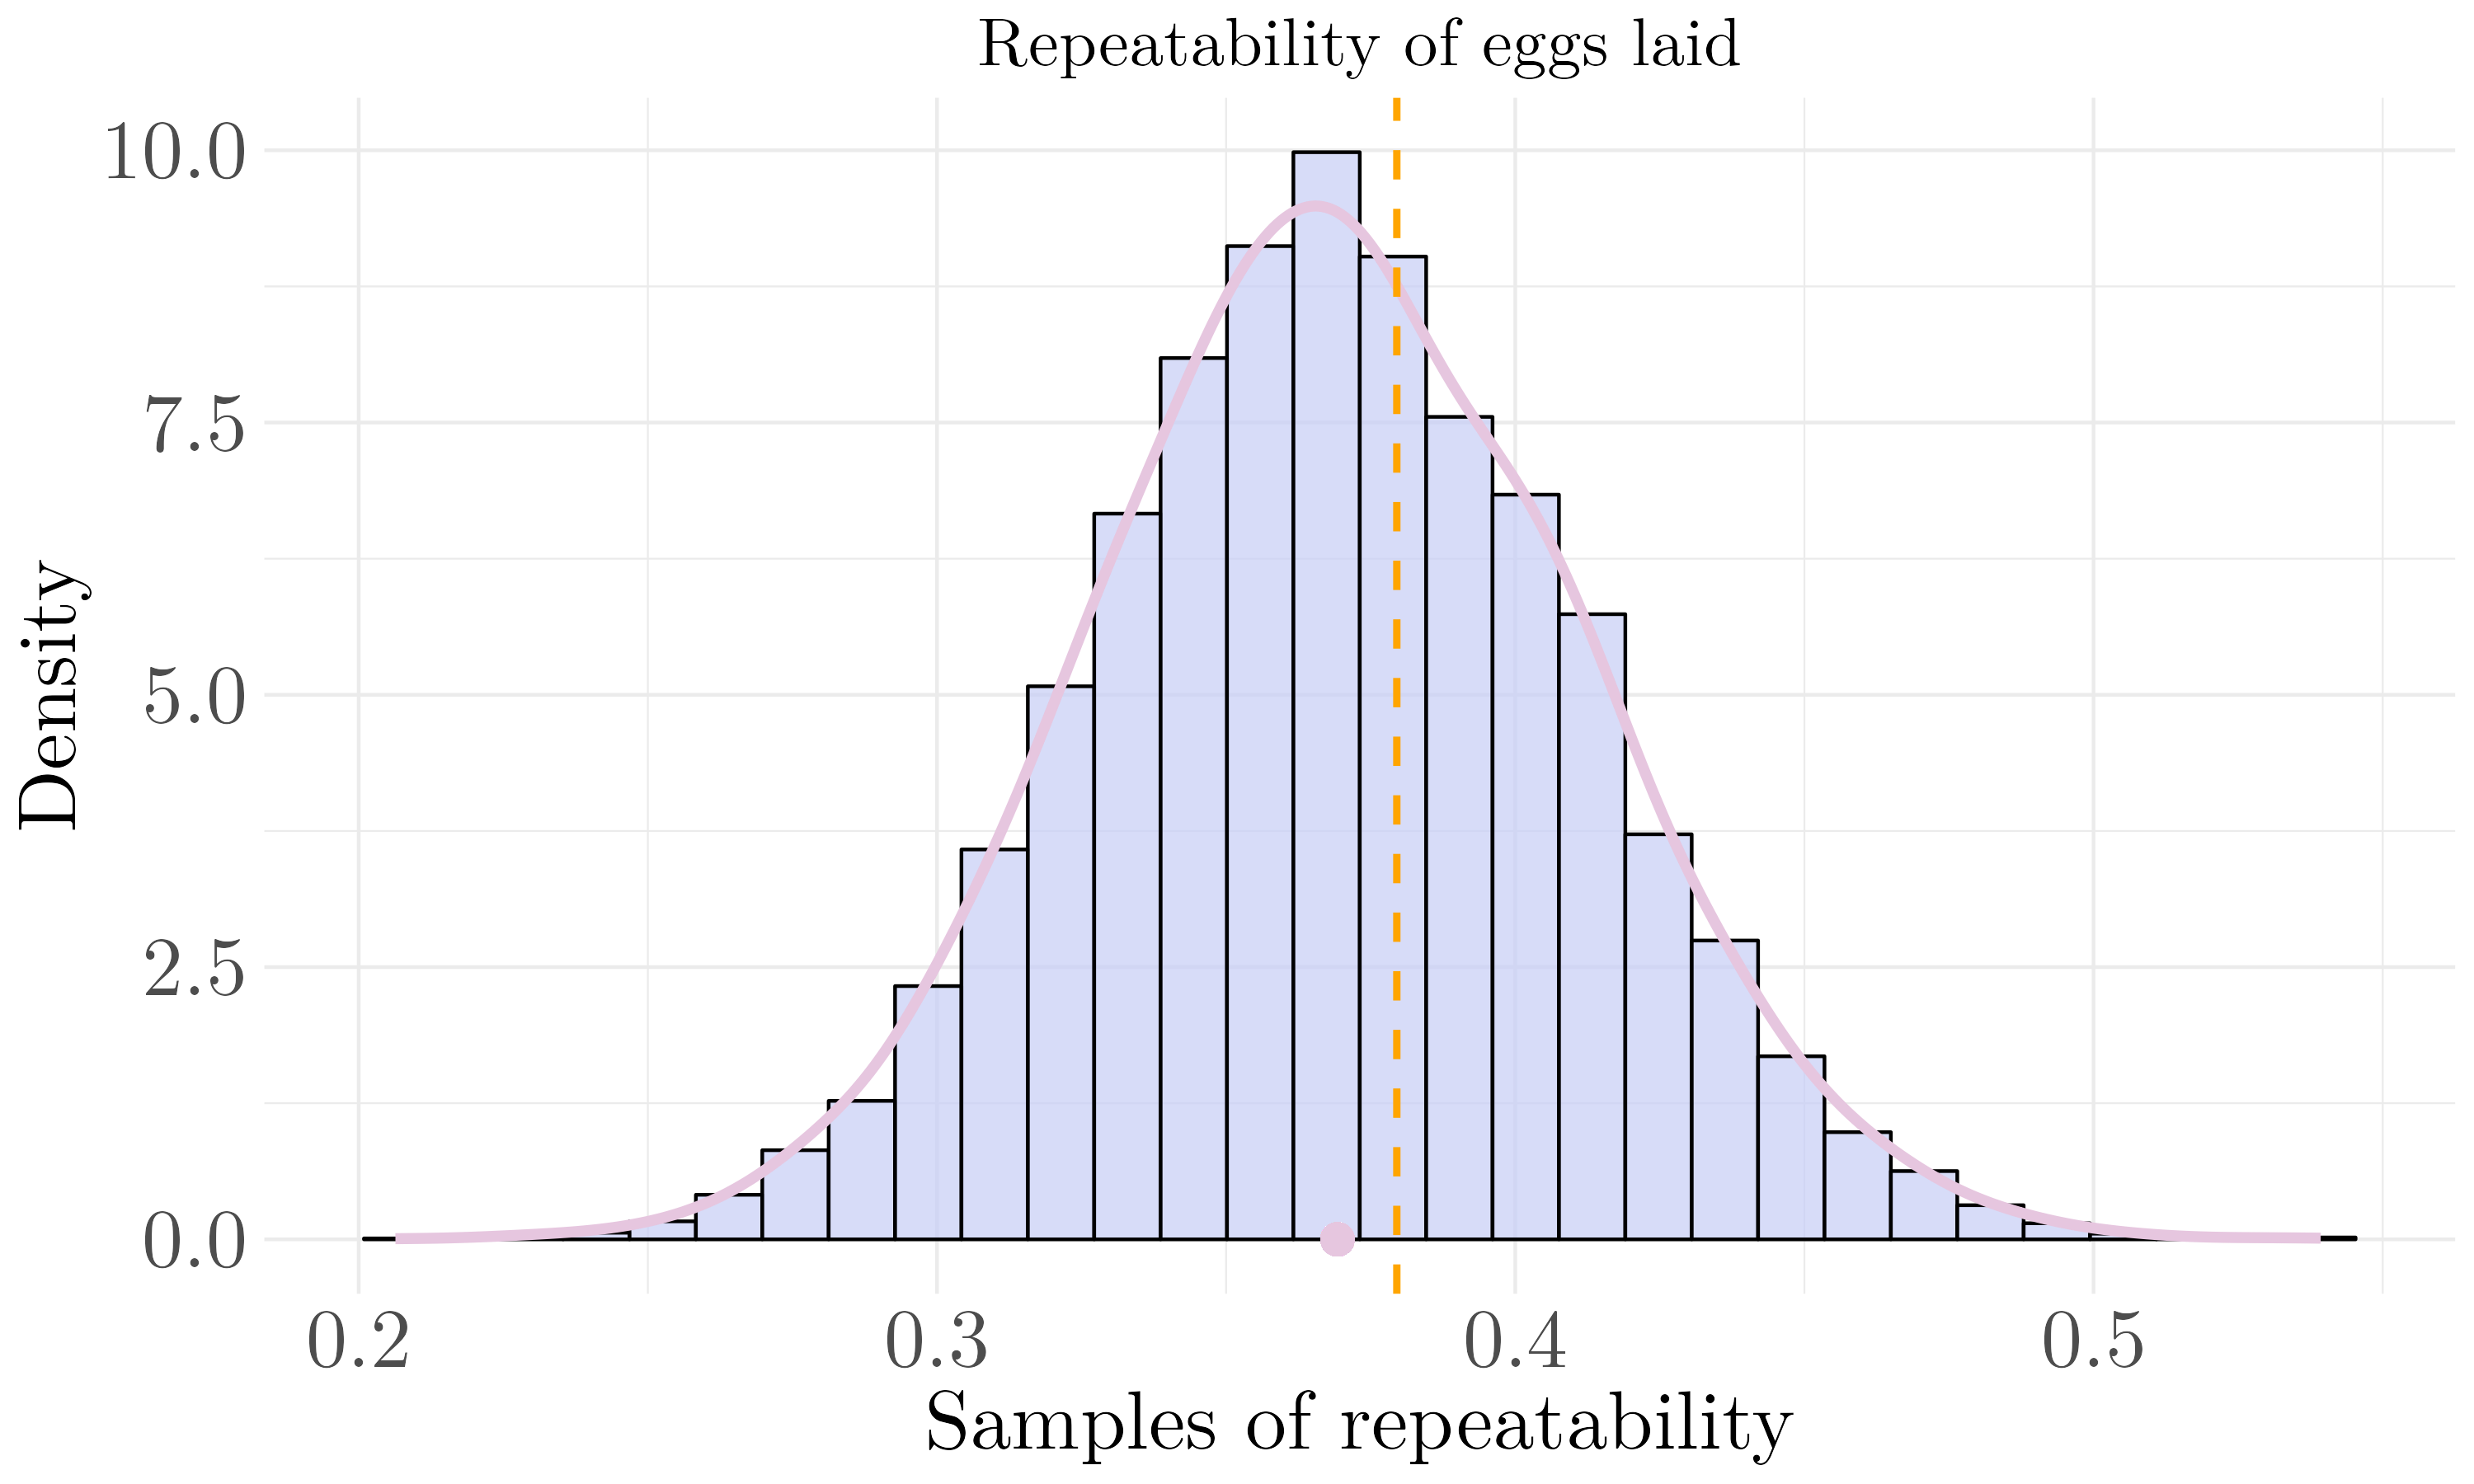
\includegraphics[width=\linewidth]{Figures/Stoffel Comparison/Heritability_egg_poisson.png}
    \label{fig:heritability_eggs_poisson}
  }
  \caption{Heritability of eggs laid by female beetles from BVI method (top) and Stoffel (bottom)}
\end{figure}


% \begin{figure}[H]
%   \centering
%   \begin{subfloat}{0.49\linewidth}
%       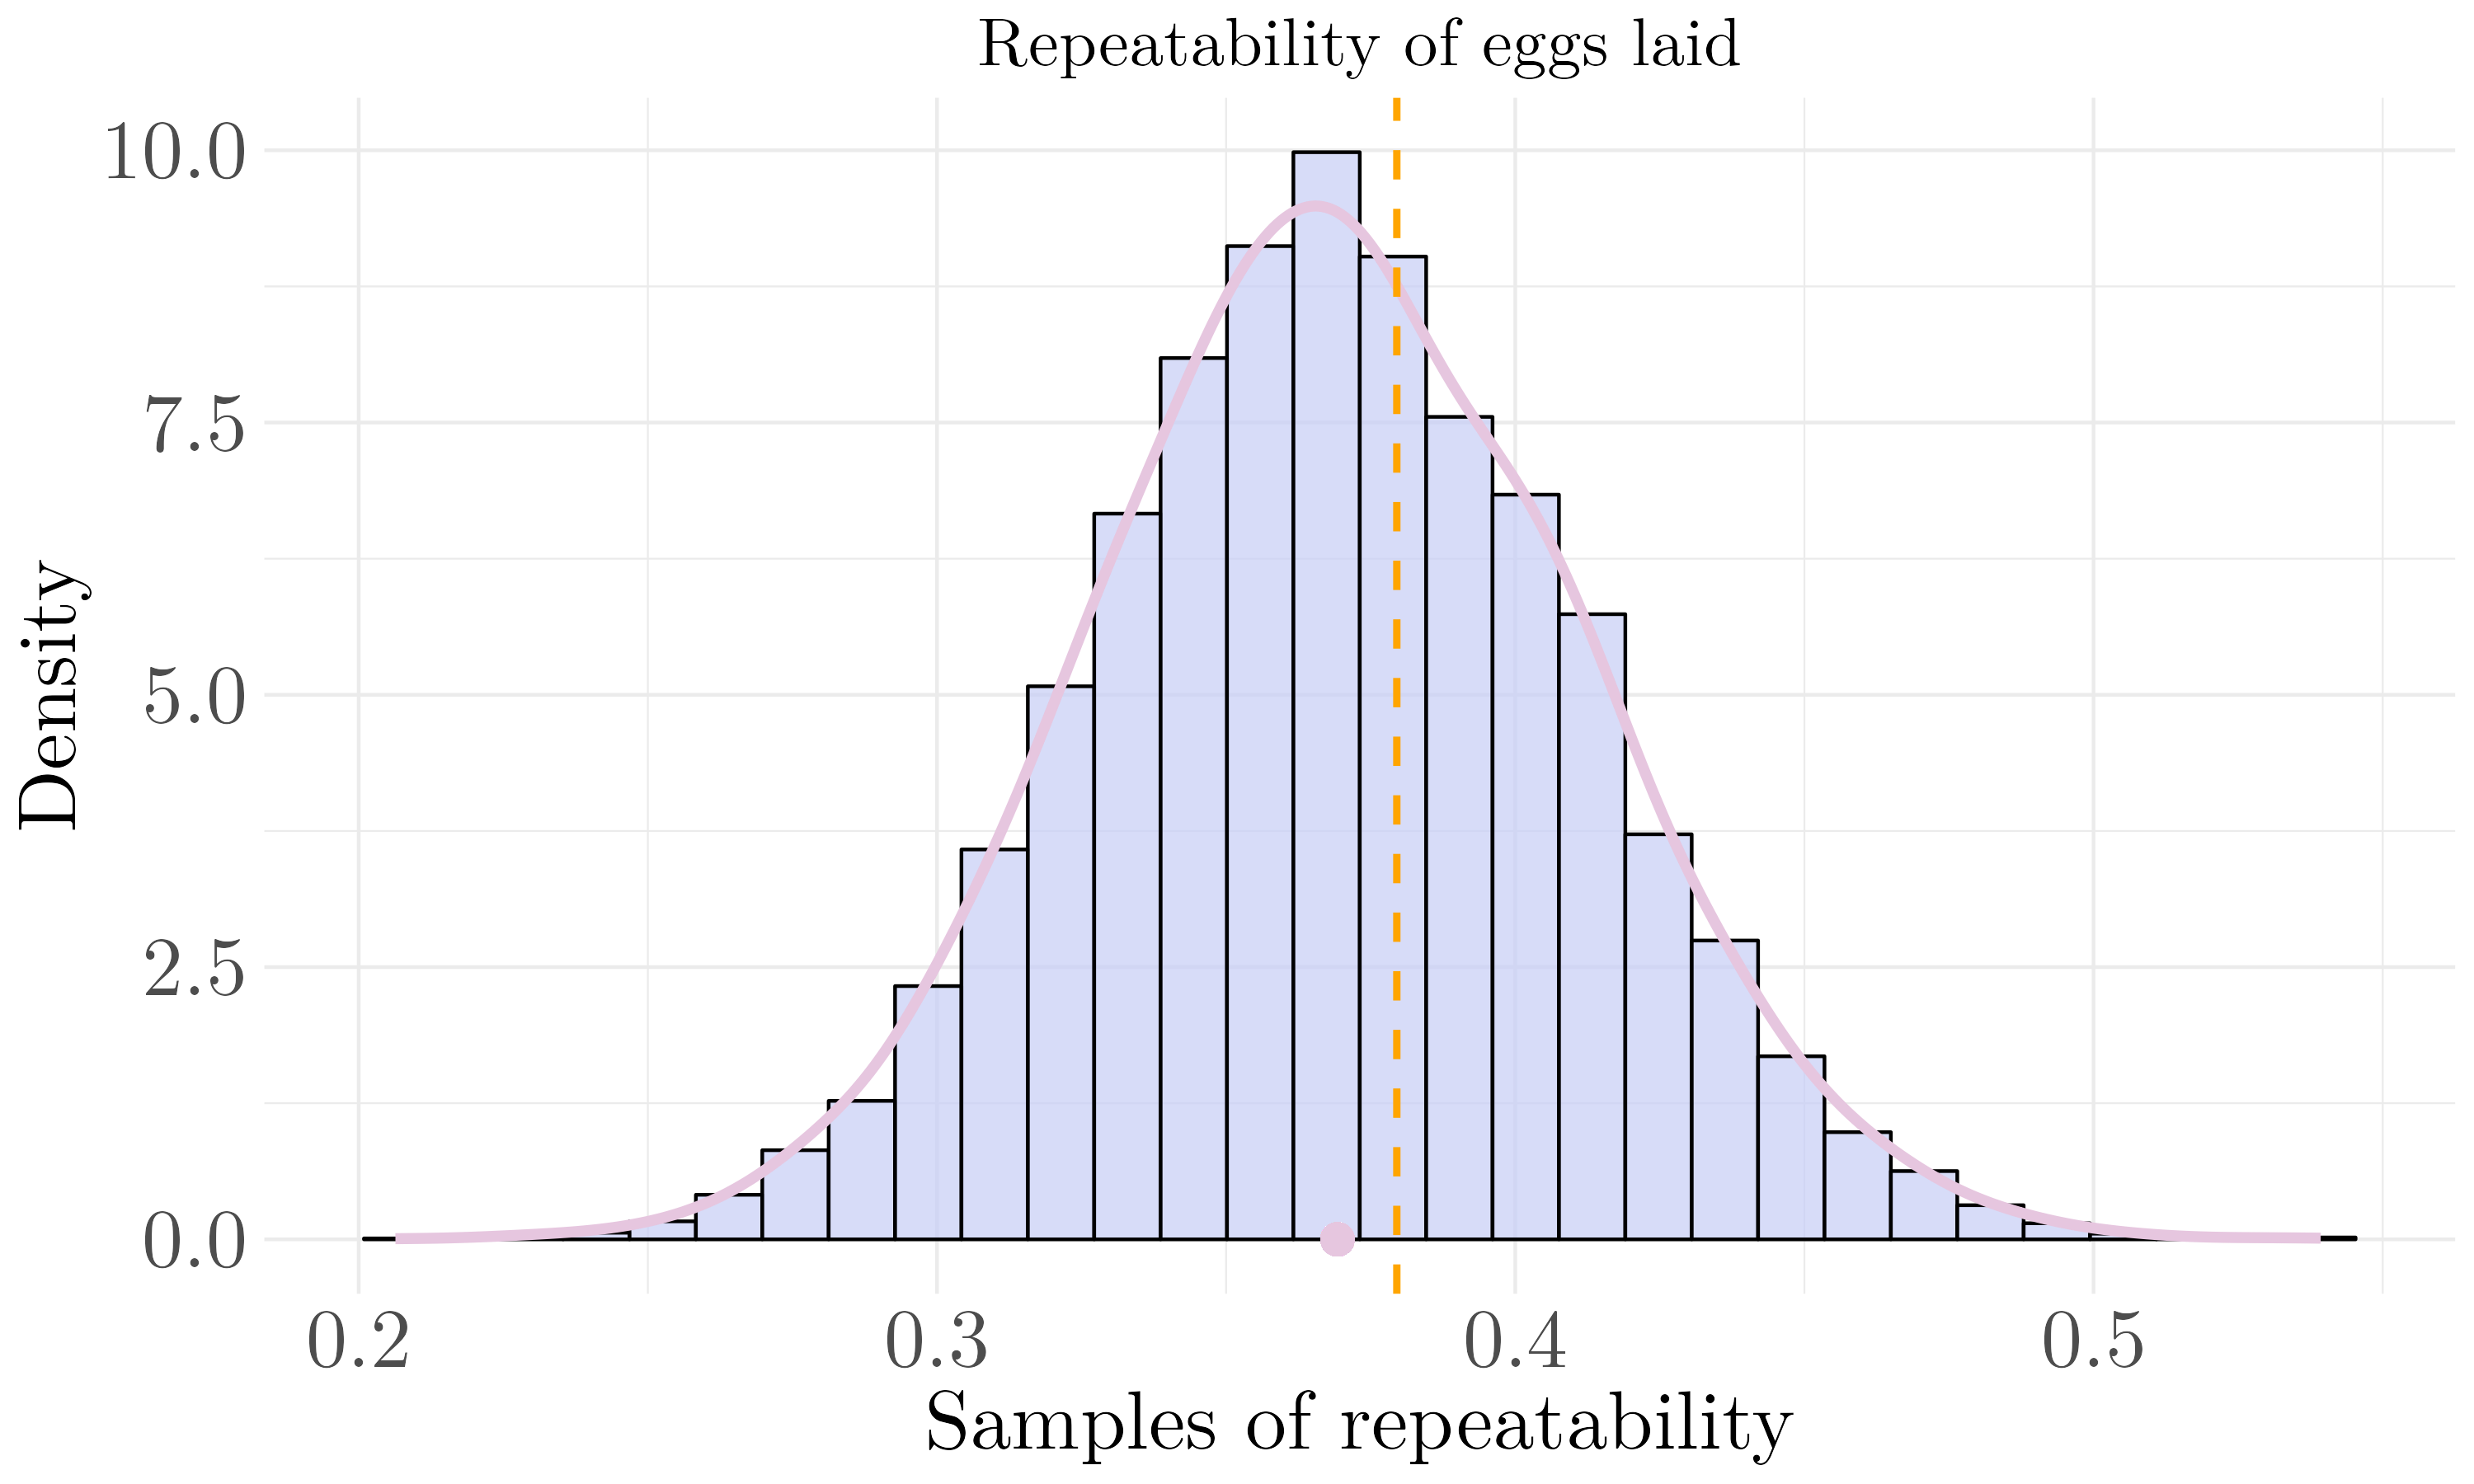
\includegraphics[width=\linewidth]{Figures/Stoffel Comparison/Heritability_egg_poisson.png}
%       \caption{Heritability of eggs laid by female beetles from BVI}
%       \label{fig:heritability_egg_poisson}
%   \end{subfloat}
%   \hfill
%   \begin{subfloat}{0.49\linewidth}
%       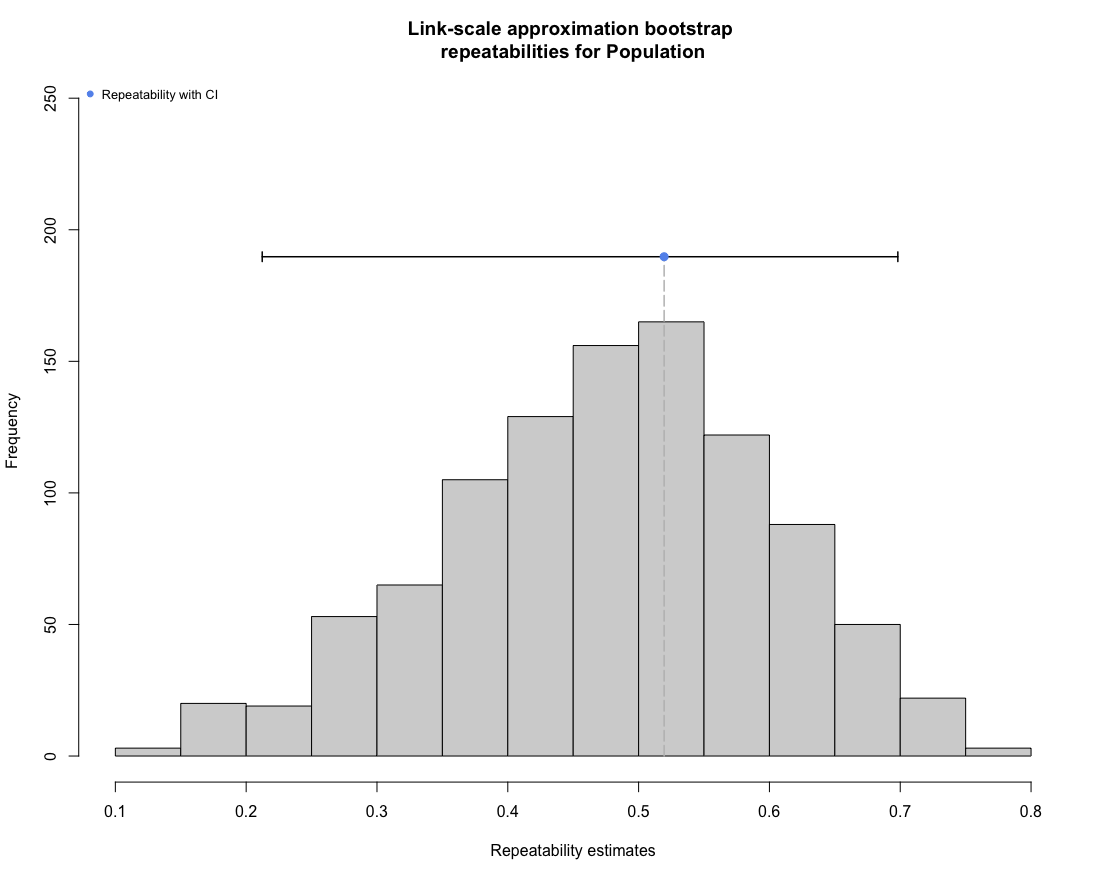
\includegraphics[width=\linewidth]{Figures/Stoffel Comparison/Heritability_egg_poisson_Stoffel.png}
%       \caption{Comparison of heritability of eggs from Stoffel}
%       \label{fig:comparison_heritability_egg}
%   \end{subfloat}
%   \caption{Heritability of eggs in female beetles and comparison}
% \end{figure}



\section{Simulation study}

\begin{table}[ht]
  \centering
  \begin{tabular}{lcccc}
  \hline
   & Binomial (logit) & Binomial (probit) & Poisson (log) \\ \hline
  Random & 0.0954 [0.0698, 0.1272] & INSERT & 0.1338 [0.1039, 0.1700] \\
  Fixed 1 & 0.0976 [0.0822, 0.1154] & INSERT & 0.1336 [0.1254, 0.1412] \\
  Fixed 2 & 0.1951 [0.1773, 0.2132] & INSERT & 0.2675 [0.2552, 0.2816] \\
  Fixed 3 & 0.2916 [0.2673, 0.3174] & INSERT & 0.4013 [0.3852, 0.4216] \\ 
  $R^2_m$ & 0.5843 [0.5545, 0.6157] & INSERT & 0.8024 [0.7697, 0.8340] \\ 
  $R^2_c$ & 0.6797 [0.6527, 0.7037] & INSERT & 0.9361 [0.9270, 0.9472] \\ \hline
  \end{tabular}
  \caption{Average relative importance across simulations using the BVI method, Stoffels results with $10$ bootstrap samples and the average expected importance (dependent on the fitted model for the Poisson model)}
  \label{tab:summary_findings}
\end{table}






% > Stoffel_logit
% [1] 0.09779636
% > Stoffel_probit
% [1] 0.1188267
% > Stoffel_pois
% [1] 0.1408853
% > Stoffel_logit_R2m
% [1] 0.5380293
% > Stoffel_logit_R2c
% [1] 0.6358256
% > Stoffel_probit_R2m
% [1] 0.7075769
% > Stoffel_probit_R2c
% [1] 0.8264035
% > Stoffel_pois_R2m
% [1] 0.8543839
% > Stoffel_pois_R2c
% [1] 0.9952691

\begin{figure}[H]
  \centering
    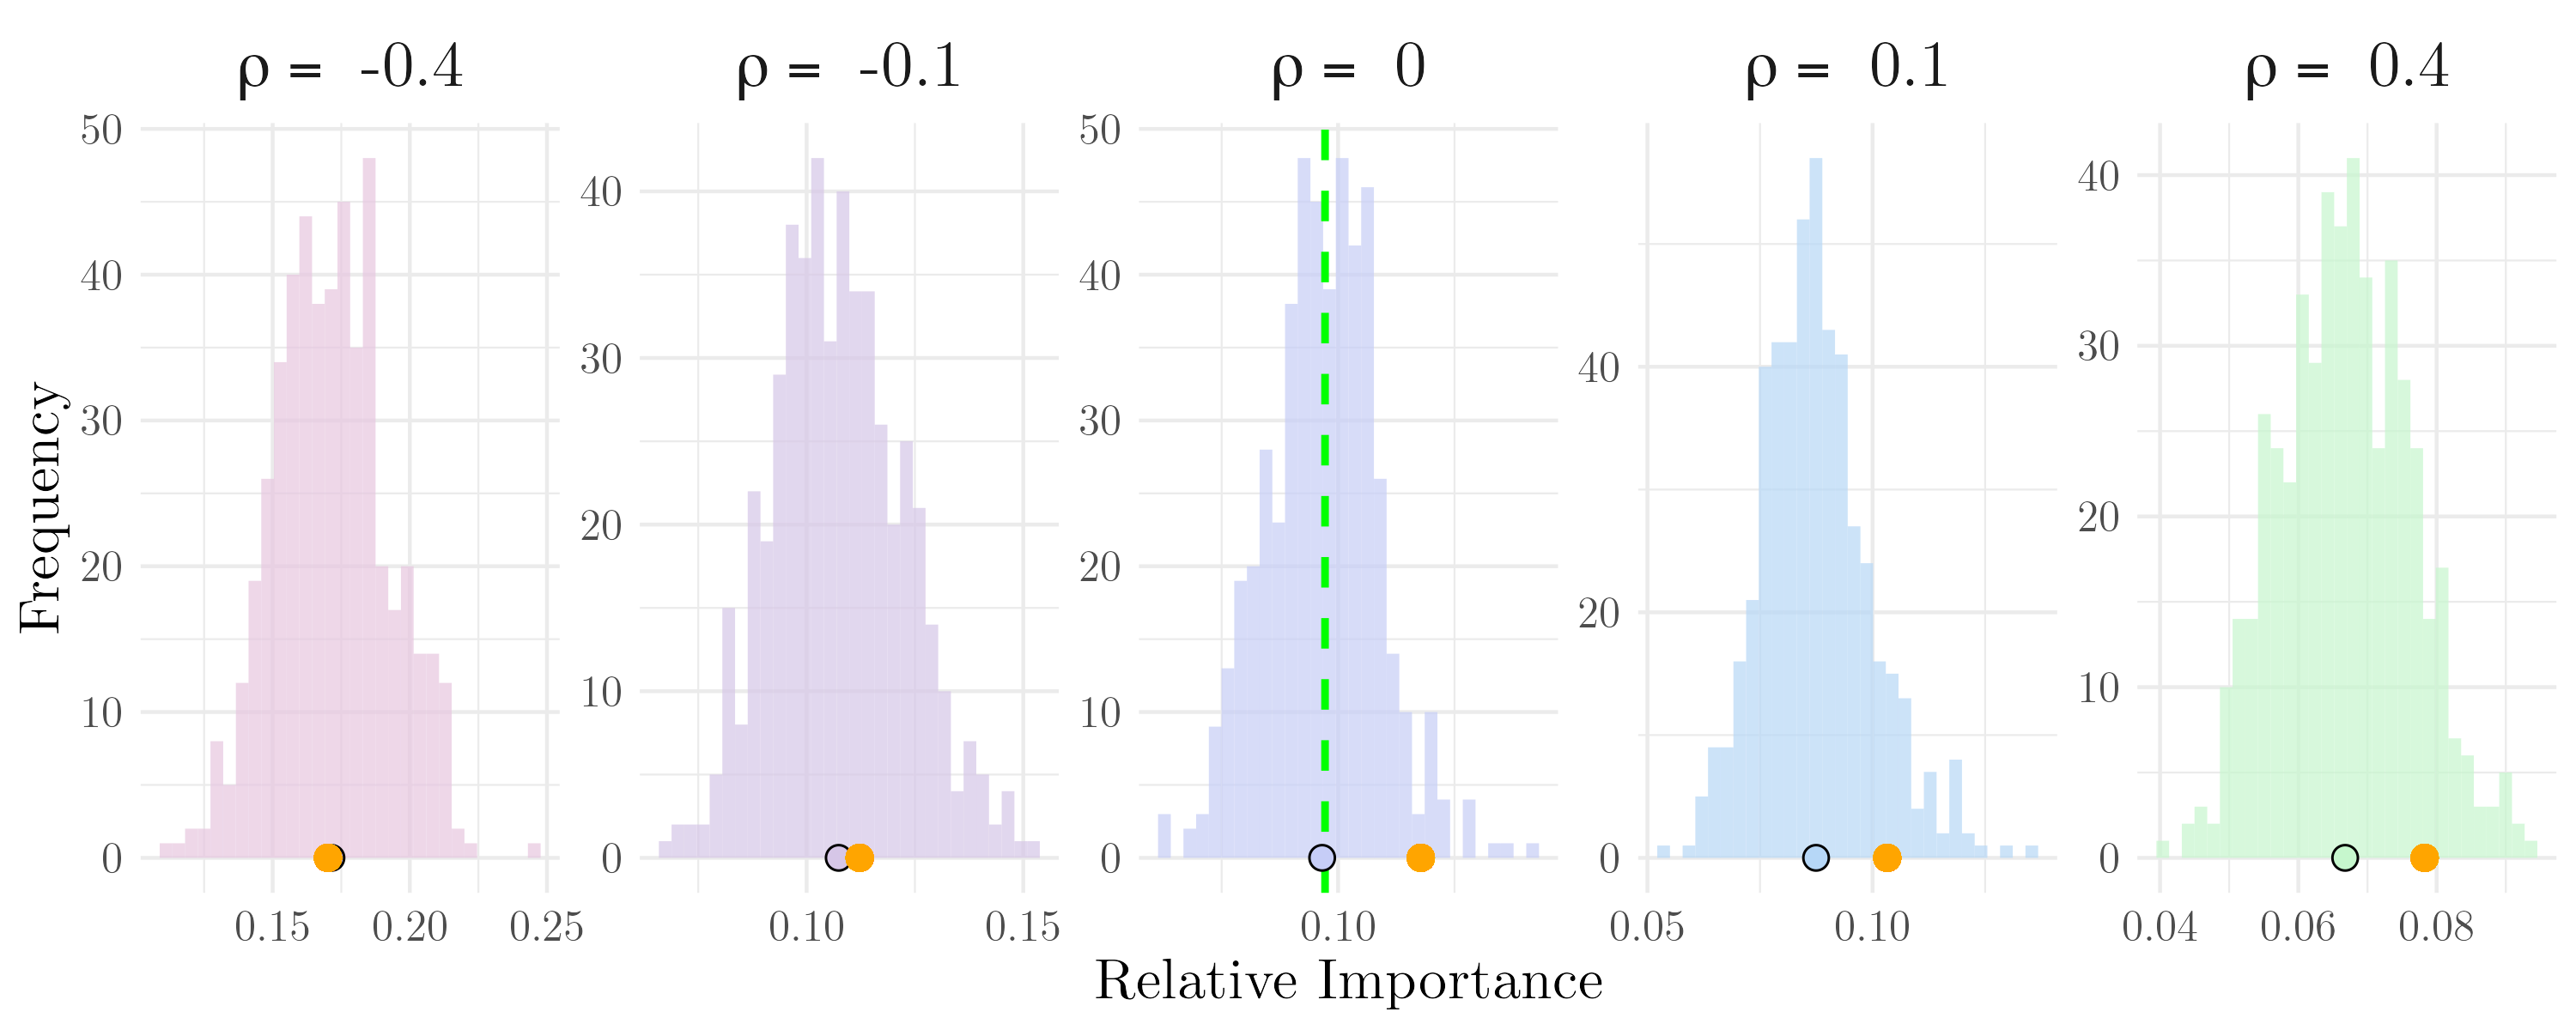
\includegraphics[width=0.7\linewidth]{Figures/Simulation study/Random_logit.png}
    \caption{Relative importance of the random effect for binomial GLMM with logit link and Poisson GLMM with log link. The magenta line is Stoffel, green line is expected importance}
    \label{fig:relimp_random_logit}
\end{figure}


\begin{figure}[H]
    \centering
      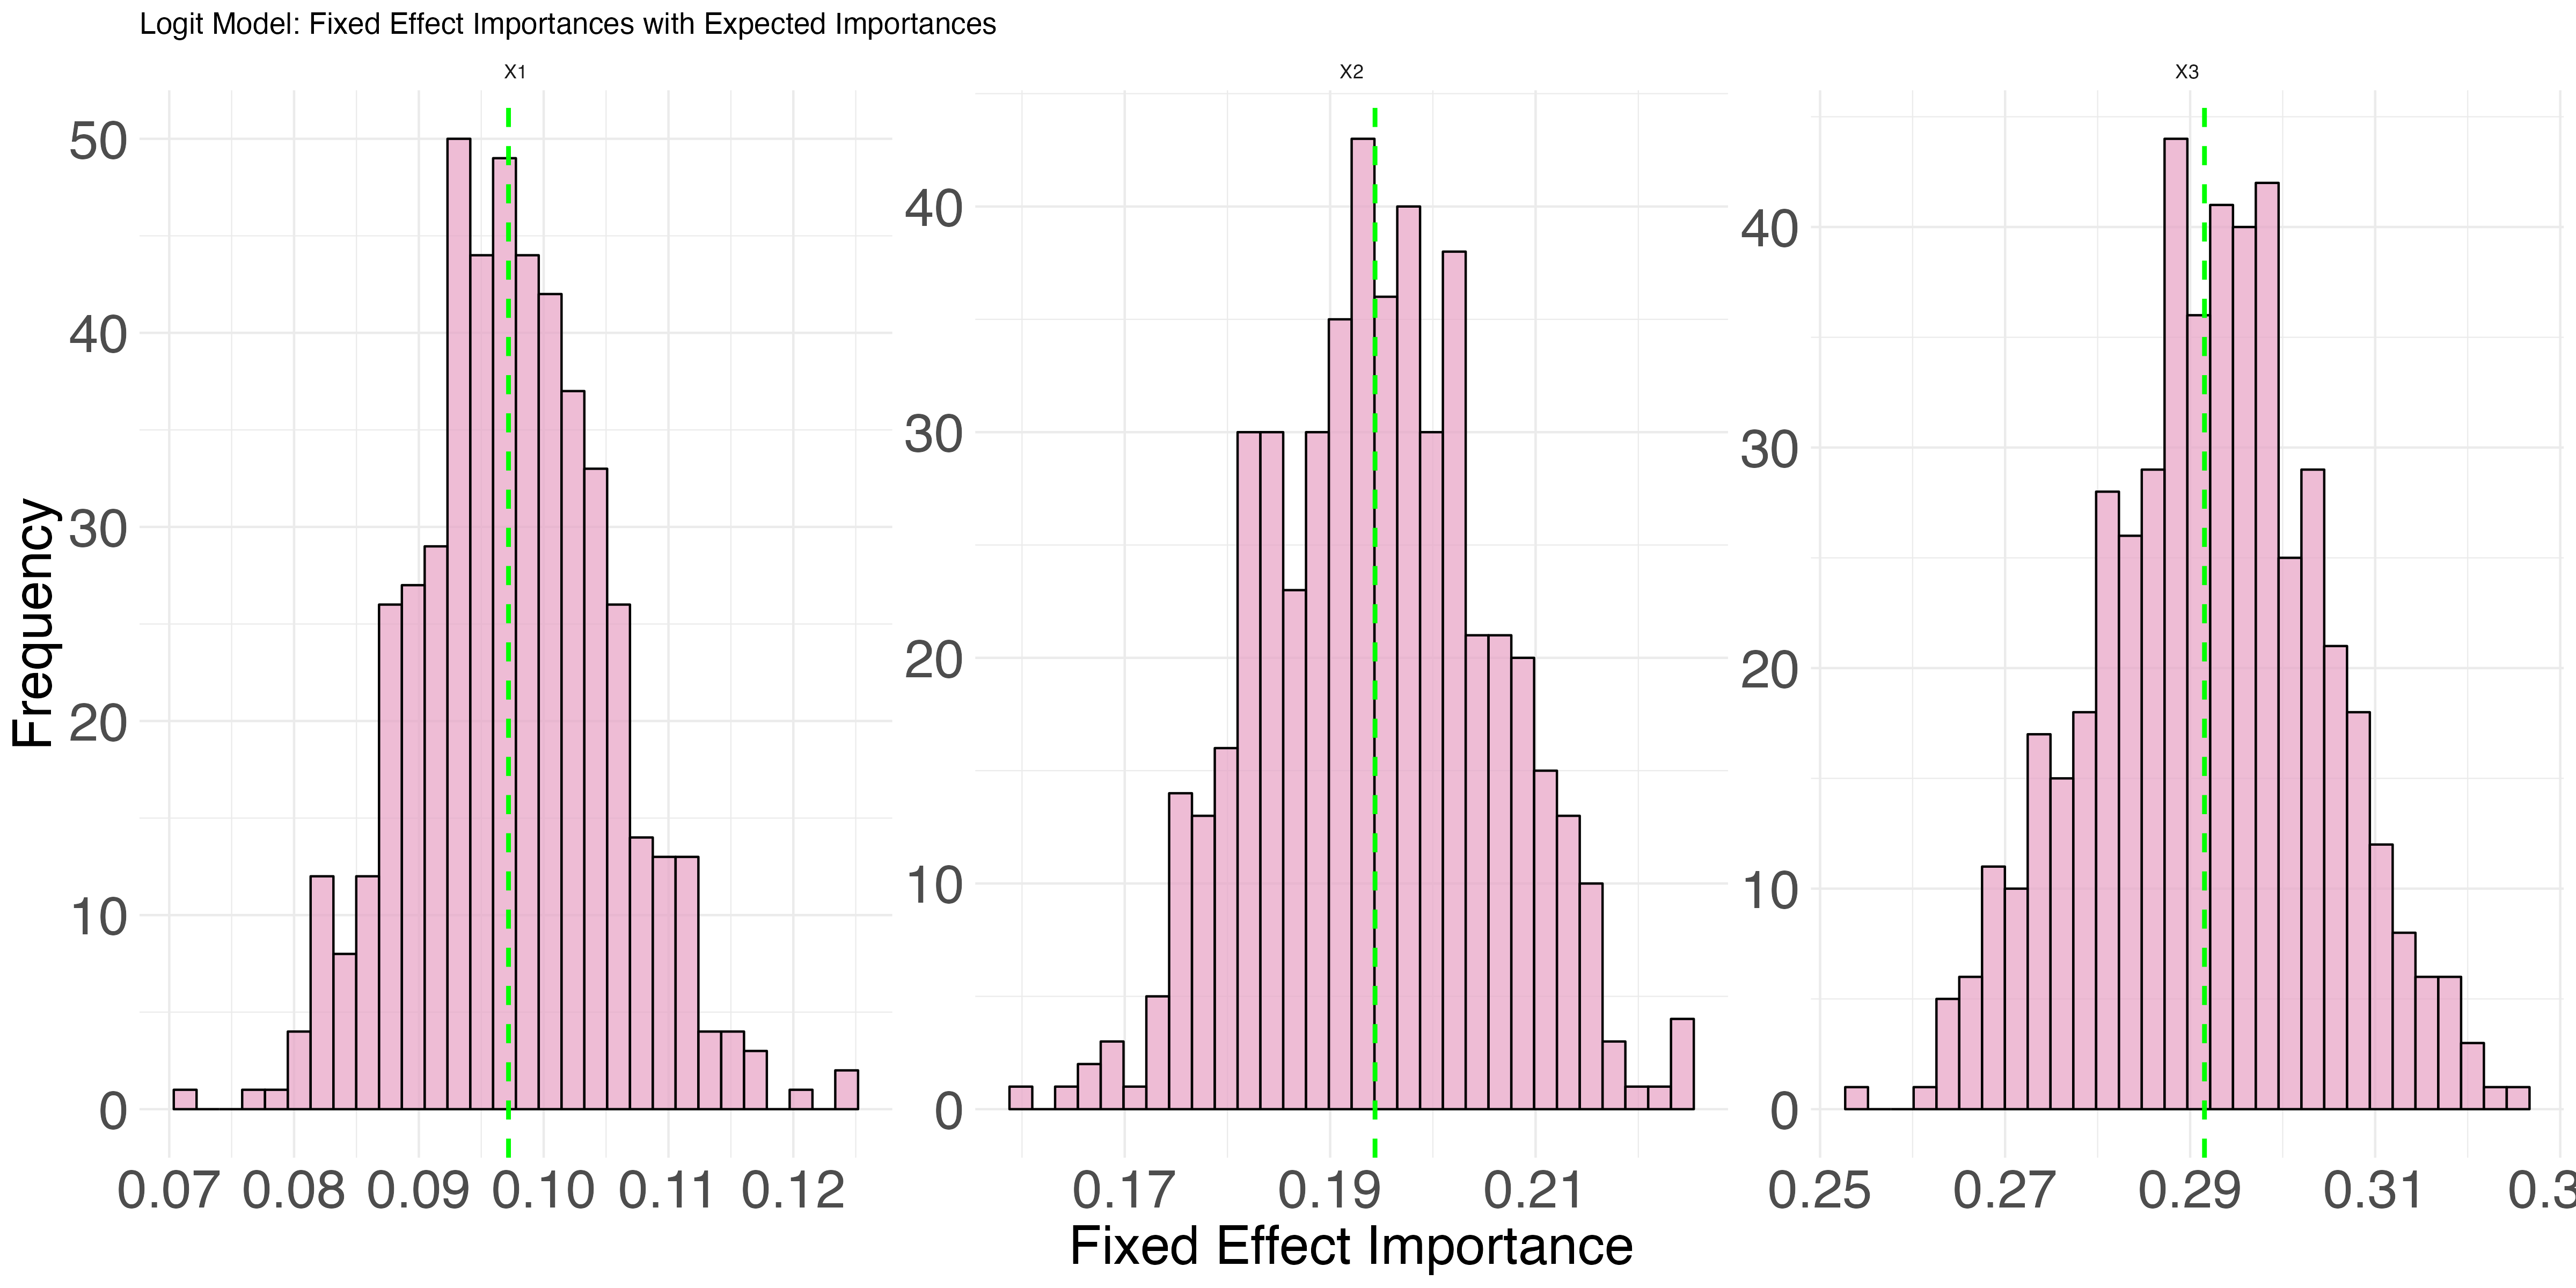
\includegraphics[width=0.7\linewidth]{Figures/Simulation study/Fixed_logit.png}
      \caption{Relative importance of fixed effects for binomial GLMM with logit link. Blue line is expected importance}
      \label{fig:relimp_binomial_logit_fixed}
  \end{figure}
  \begin{figure}[H]\ContinuedFloat
    \centering
    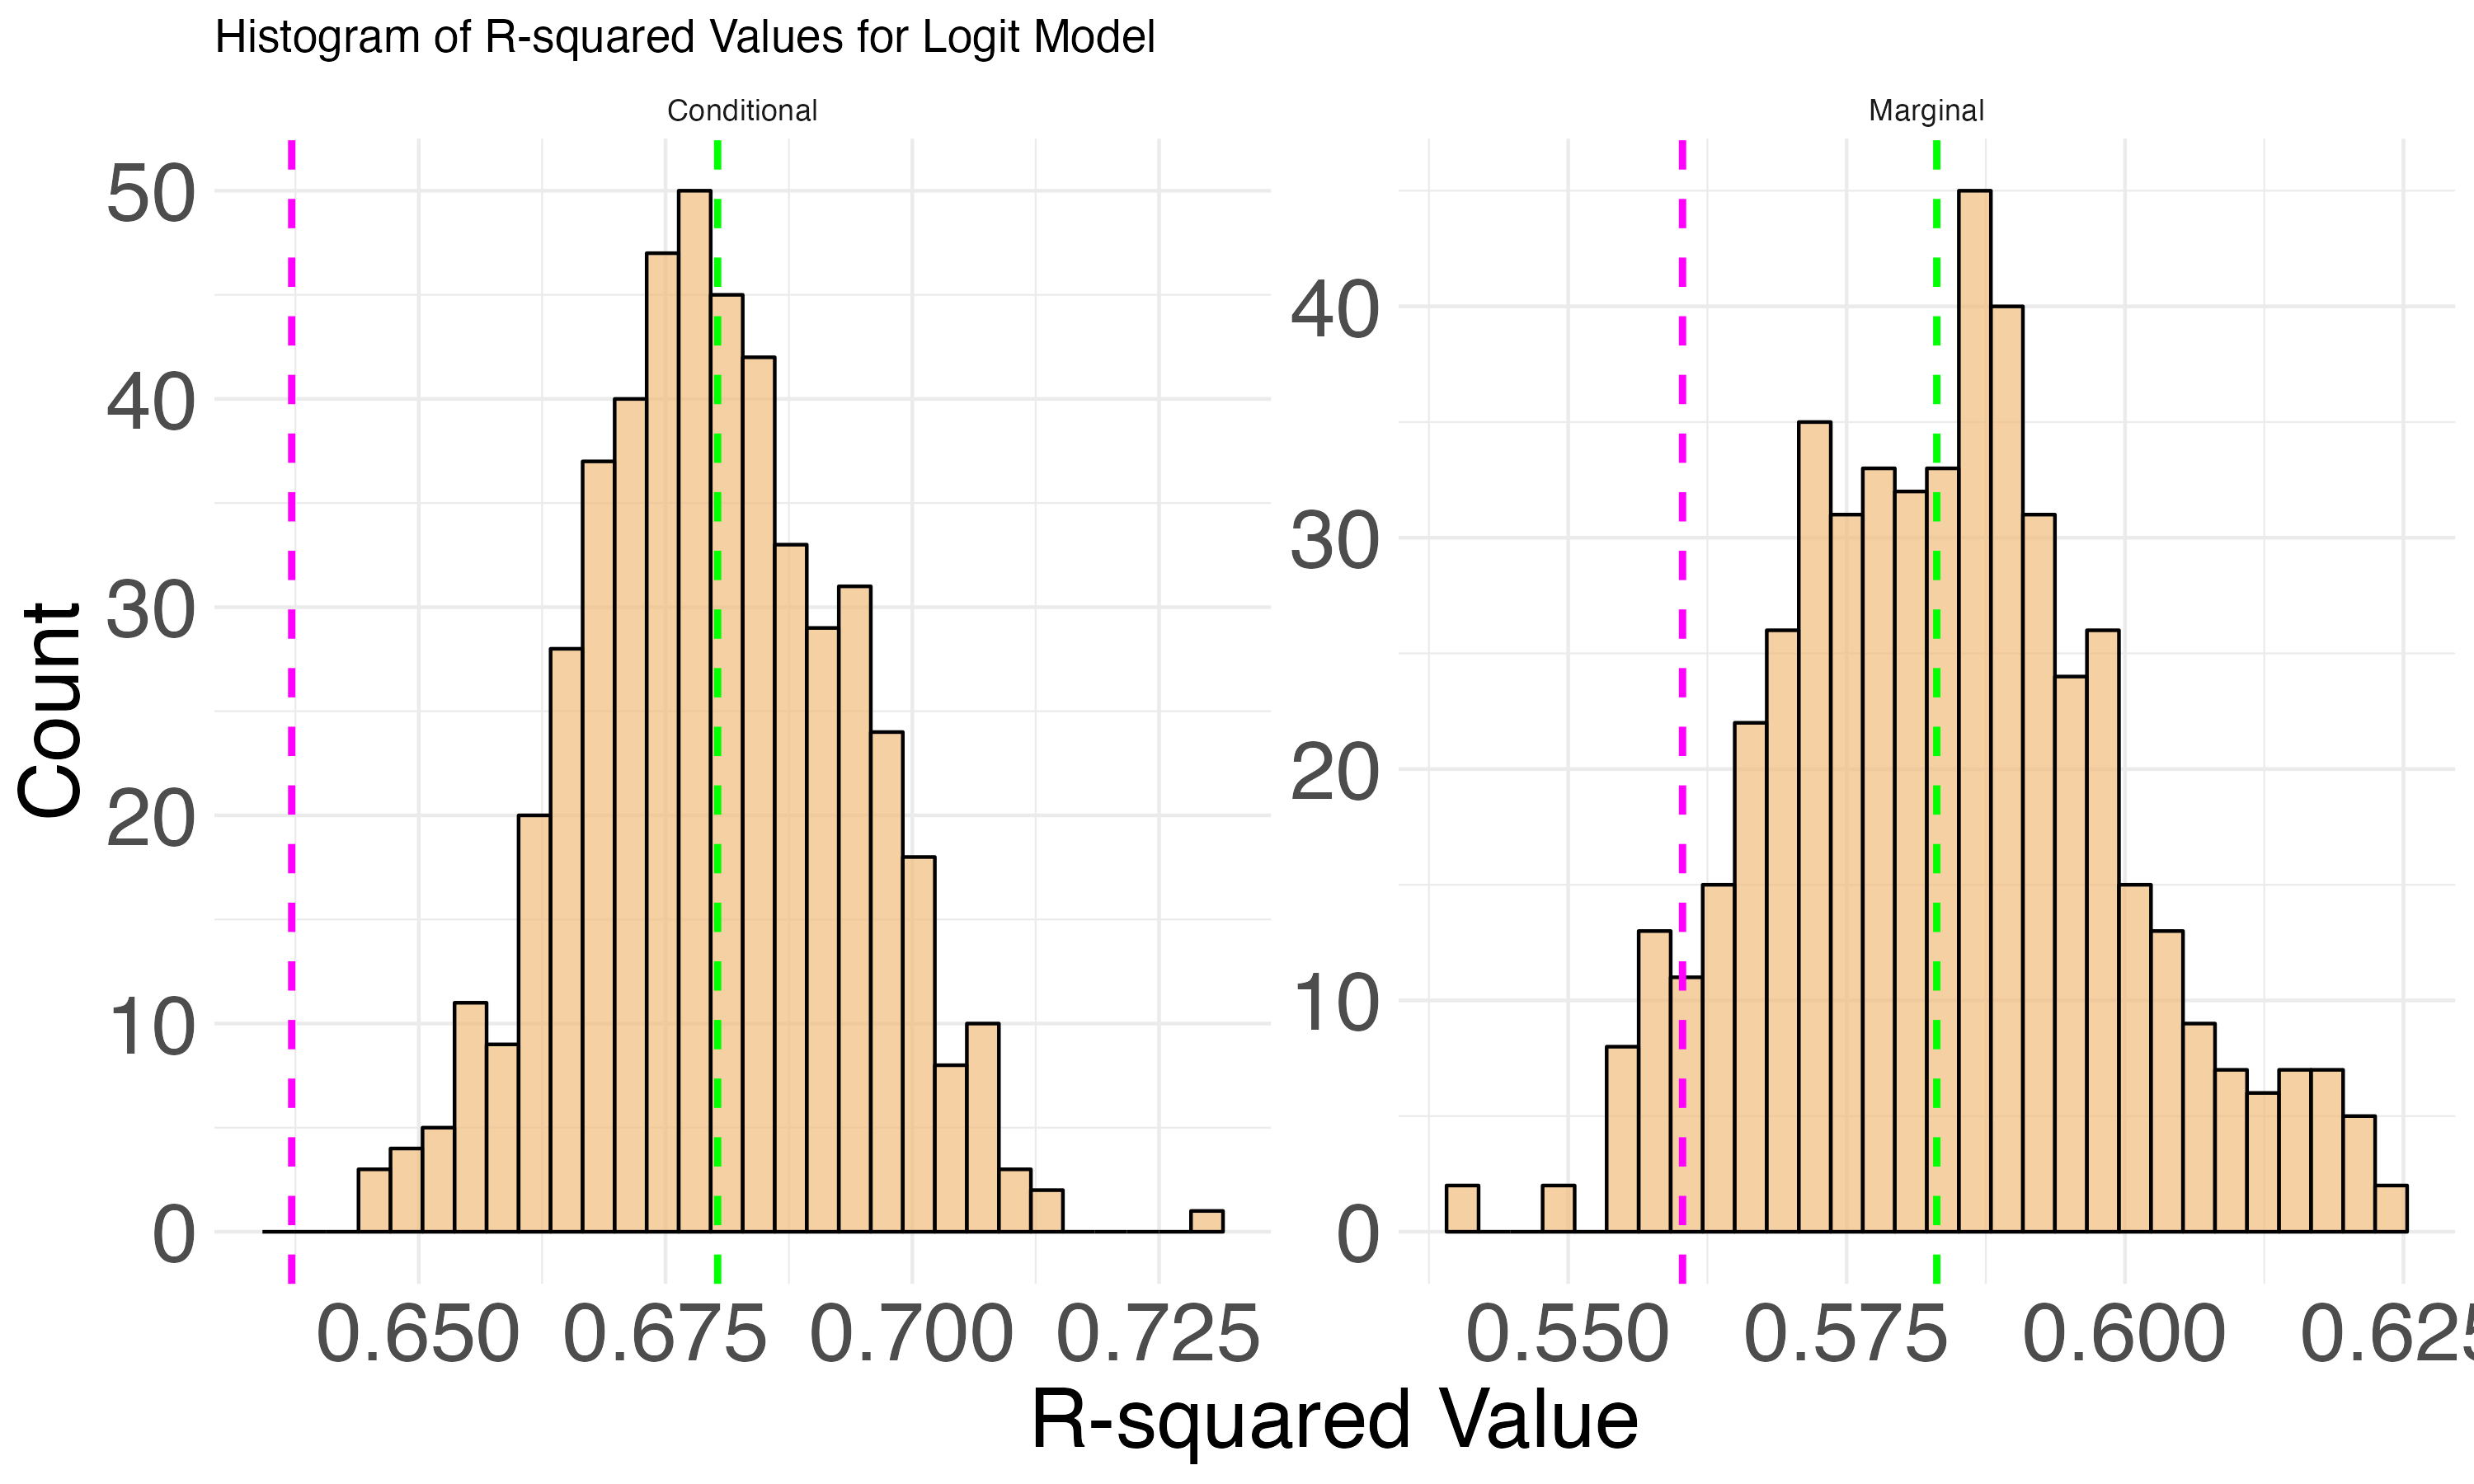
\includegraphics[width=0.7\linewidth]{Figures/Simulation study/R2_logit.png}
    \caption{Conditional and marginal $R^2$ for binomial GLMM with logit link. The magenta line is Stoffel, green line is expected importance}
      \label{fig:relimp_binomial_logit_r2}
  \end{figure}

  % \begin{figure}[H]
  %   \centering
  %     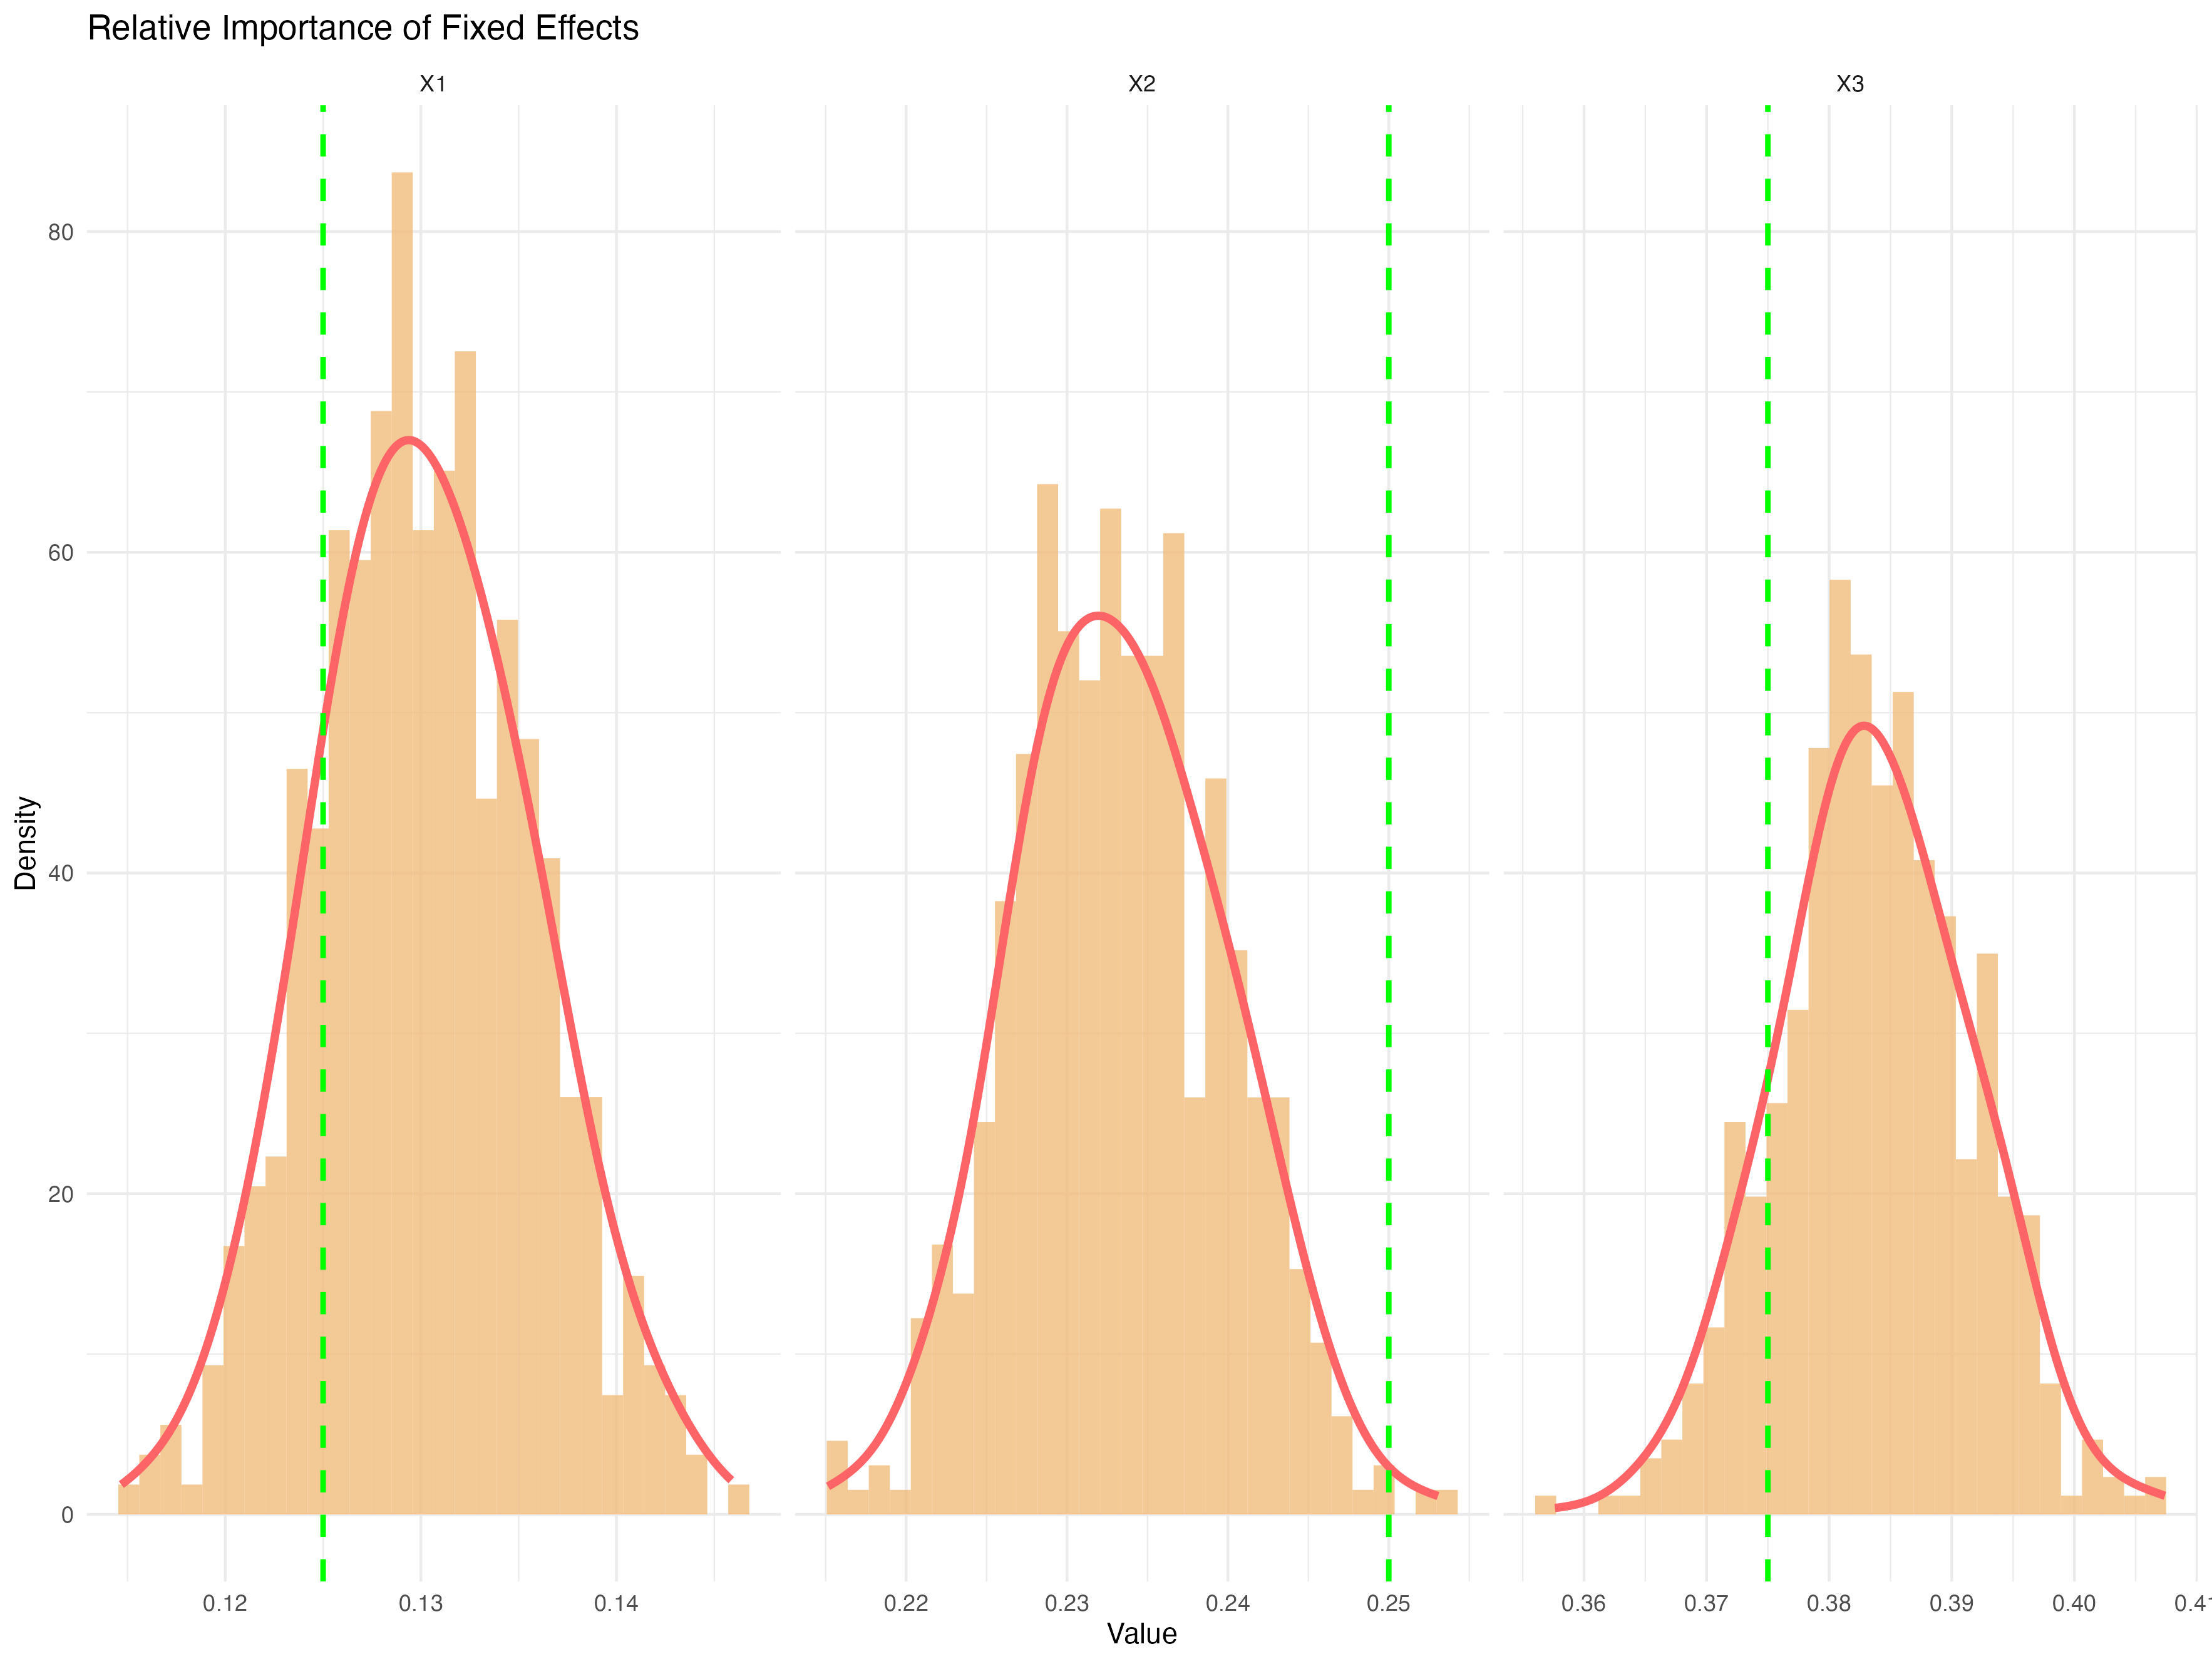
\includegraphics[width=0.7\linewidth]{Figures/Simulation study/Binomial_probit_fixed.png}
  %     \caption{Relative importance of fixed effects for binomial GLMM with probit link}
  %     \label{fig:relimp_binomial_probit_fixed}
  % \end{figure}
  % \begin{figure}[H]\ContinuedFloat
  %   \centering
  %   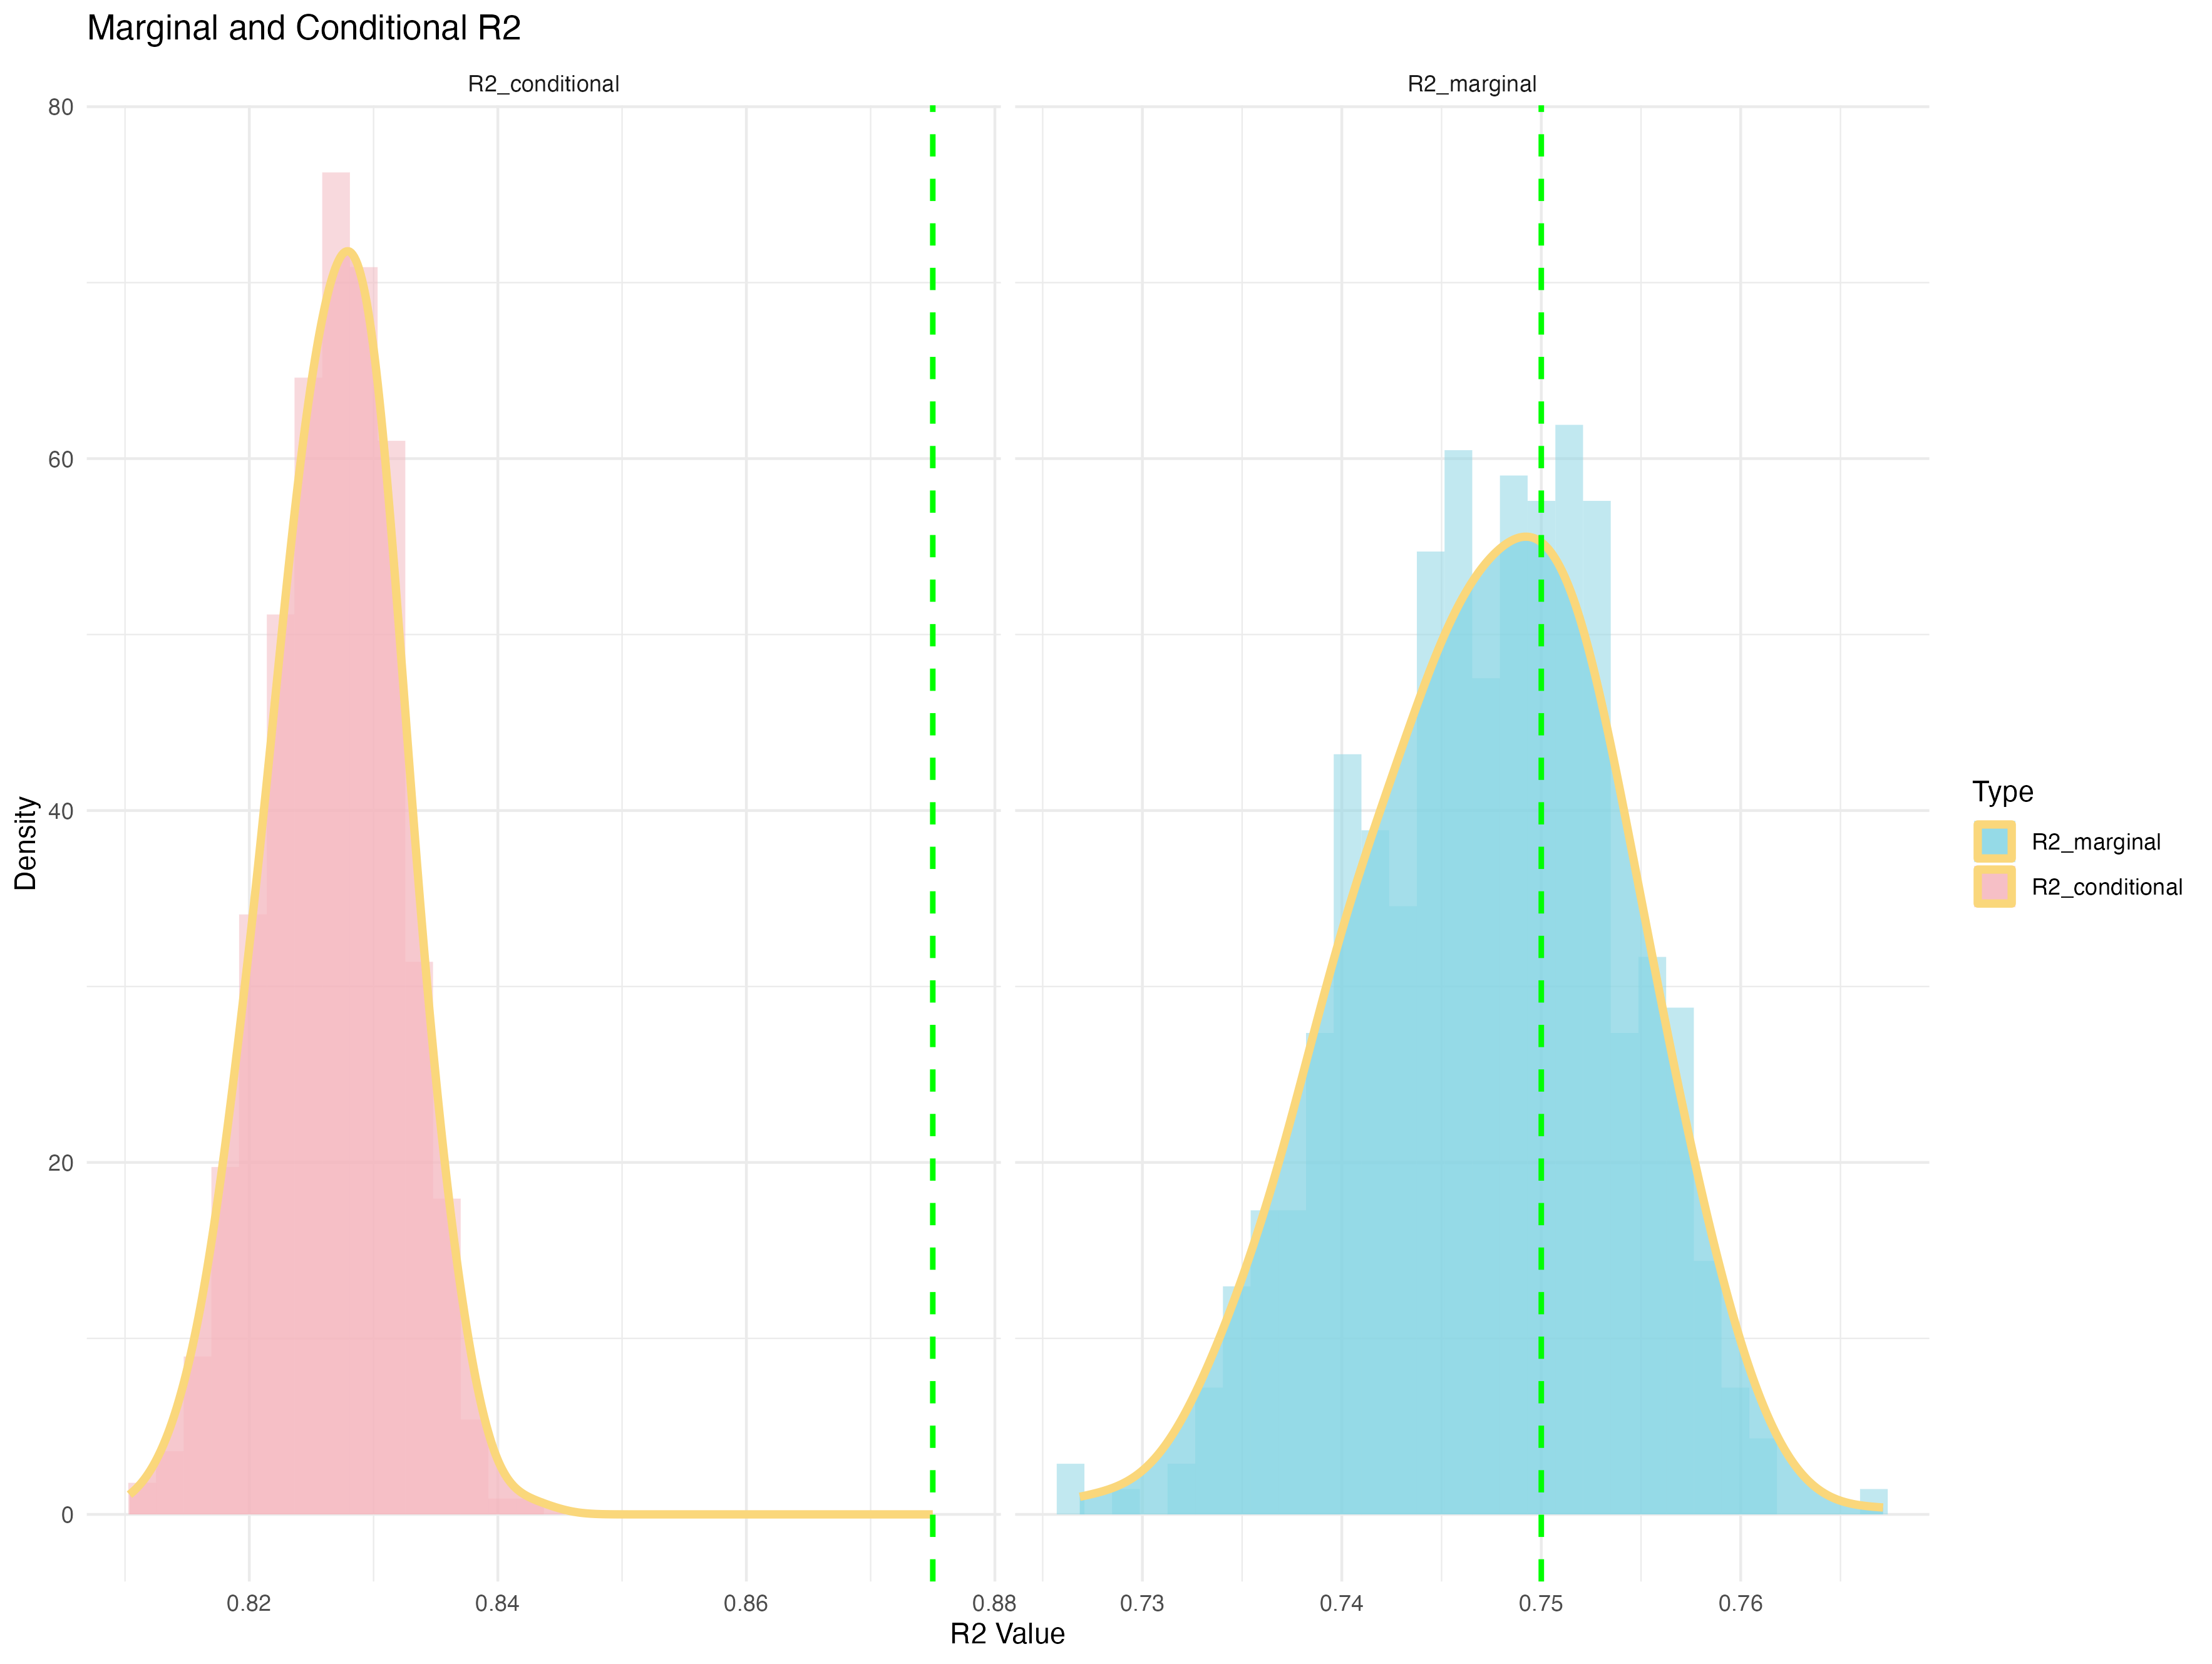
\includegraphics[width=0.7\linewidth]{Figures/Simulation study/Binomial_probit_R2.png}
  %   \caption{Conditional and marginal $R^2$ for binomial GLMM with probit link}
  %     \label{fig:relimp_binomial_probit_r2}
  % \end{figure}

\begin{figure}[H]
  \centering
    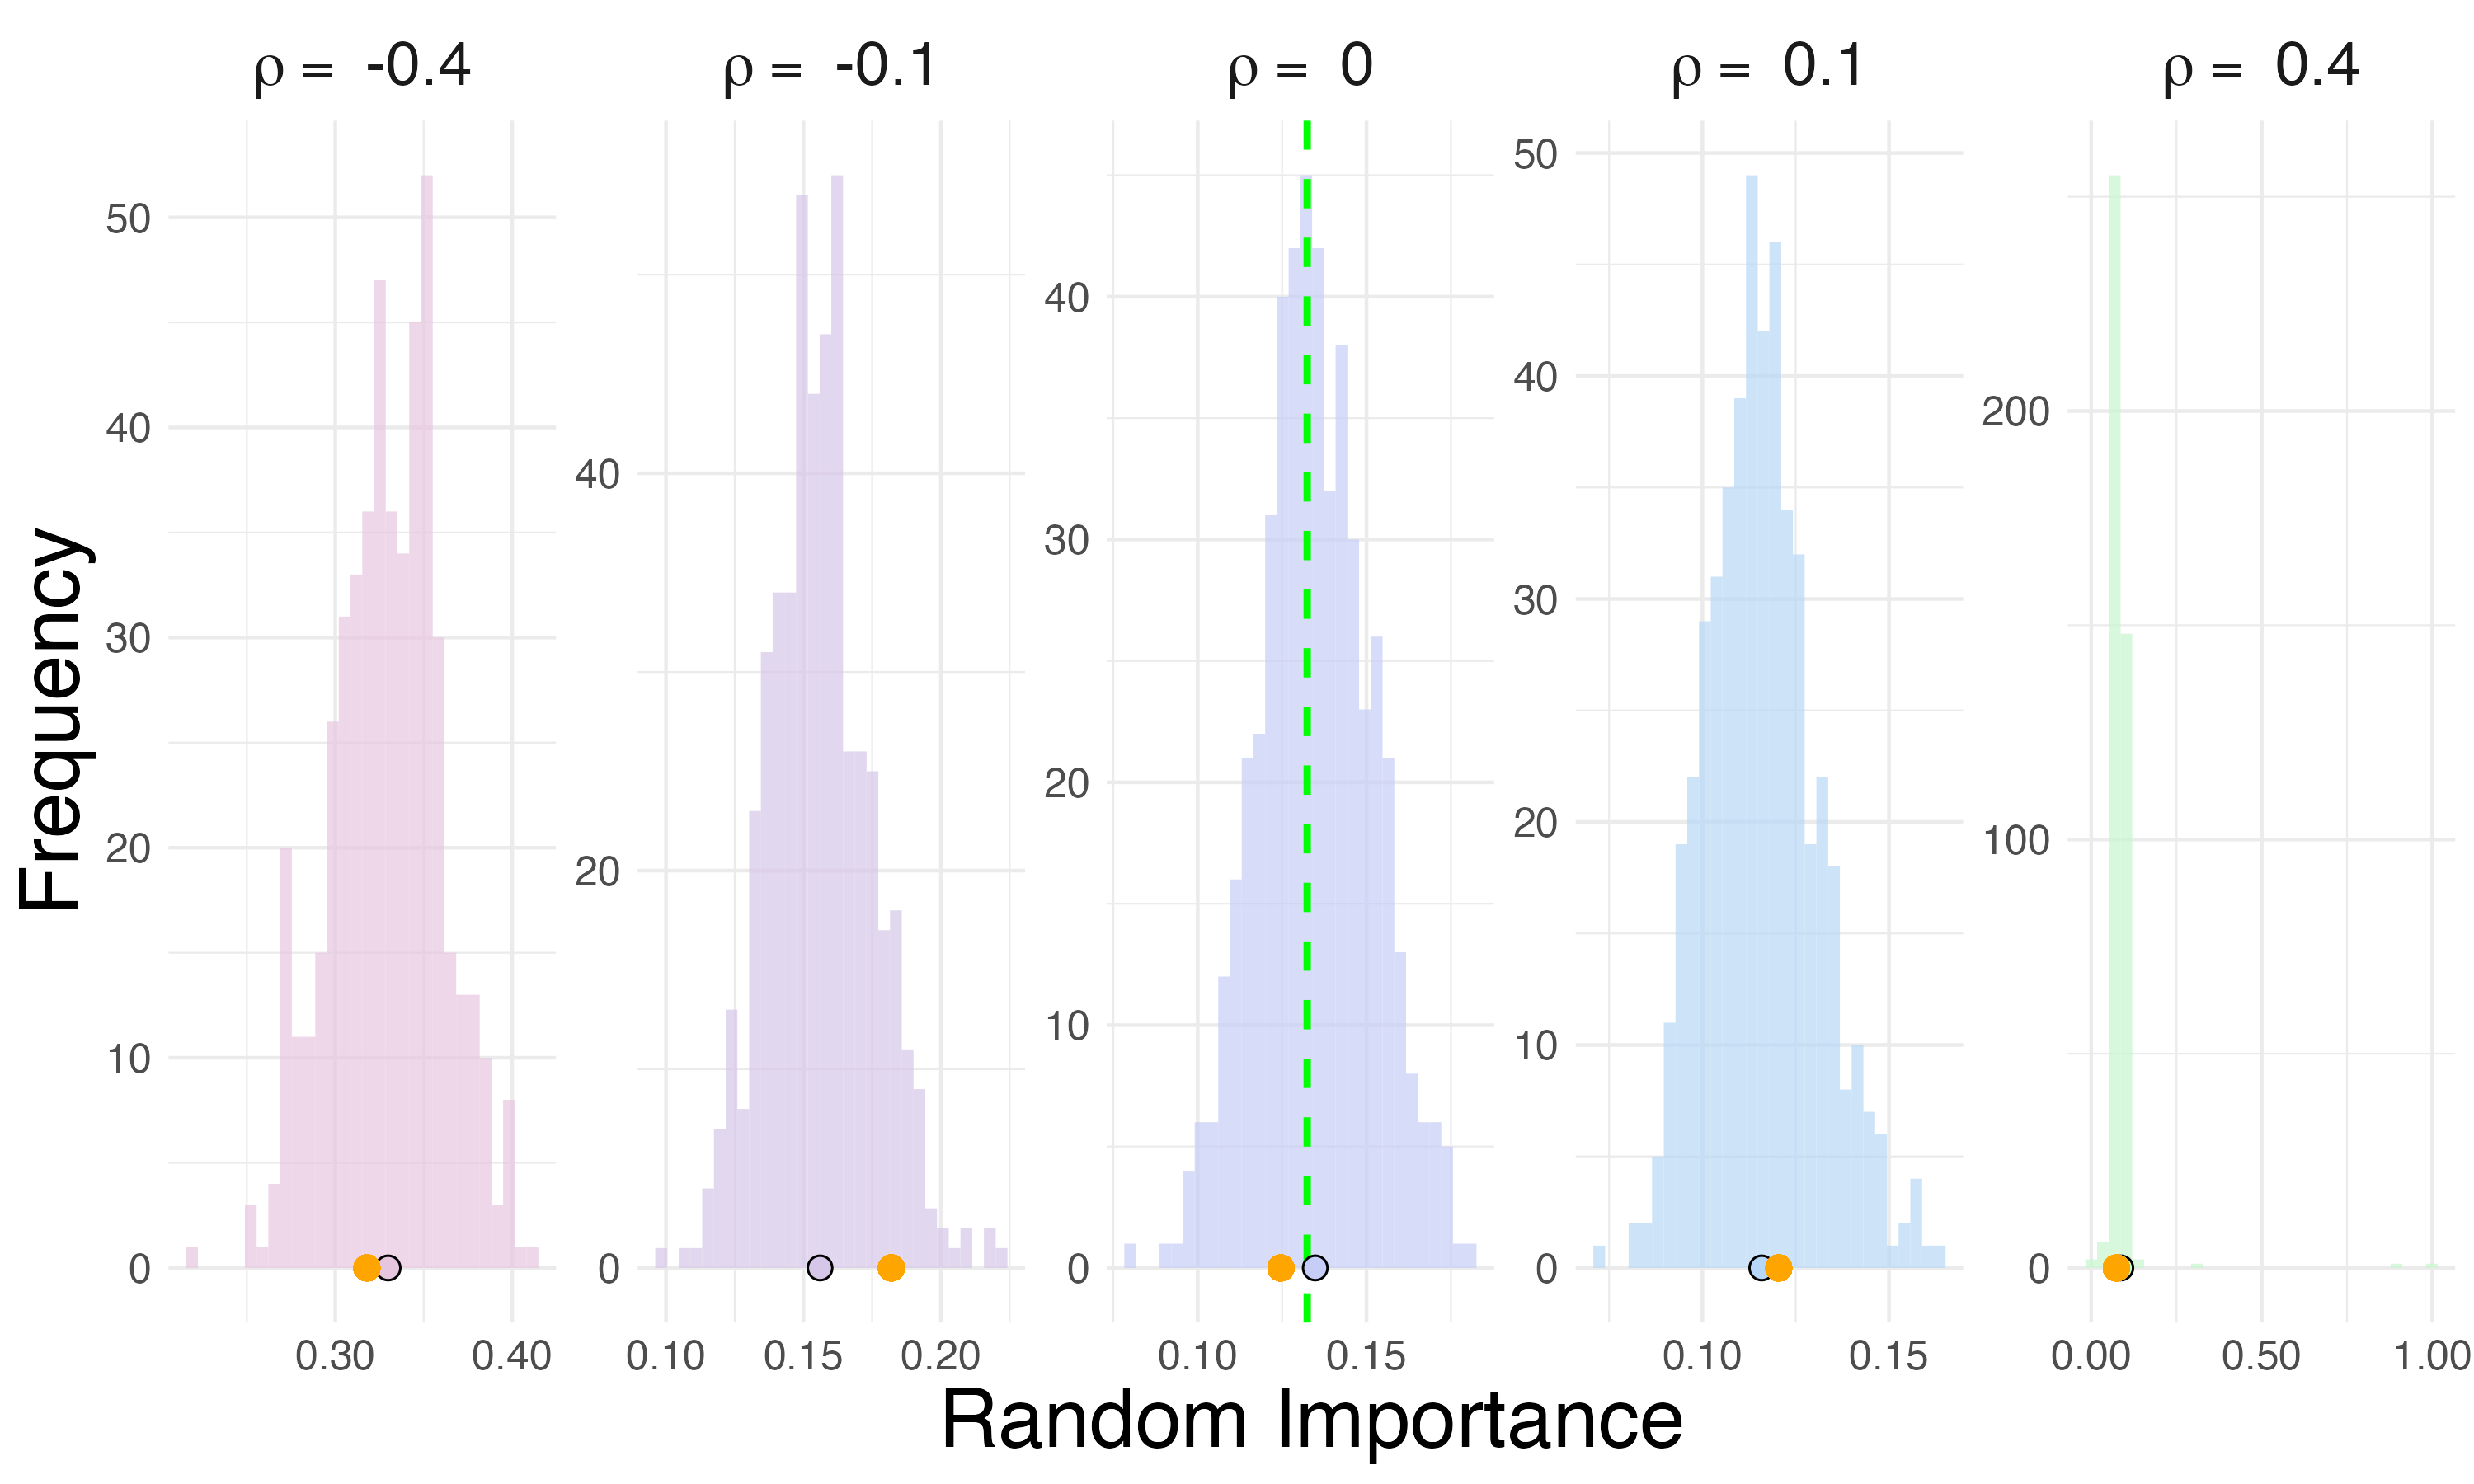
\includegraphics[width=0.7\linewidth]{Figures/Simulation study/Random_poisson.png}
    \caption{Relative importance of the random effect for binomial GLMM with logit link and Poisson GLMM with log link. The magenta line is Stoffel, green line is expected importance}
    \label{fig:relimp_random_poisson}
\end{figure}

\begin{figure}[H]
  \centering
    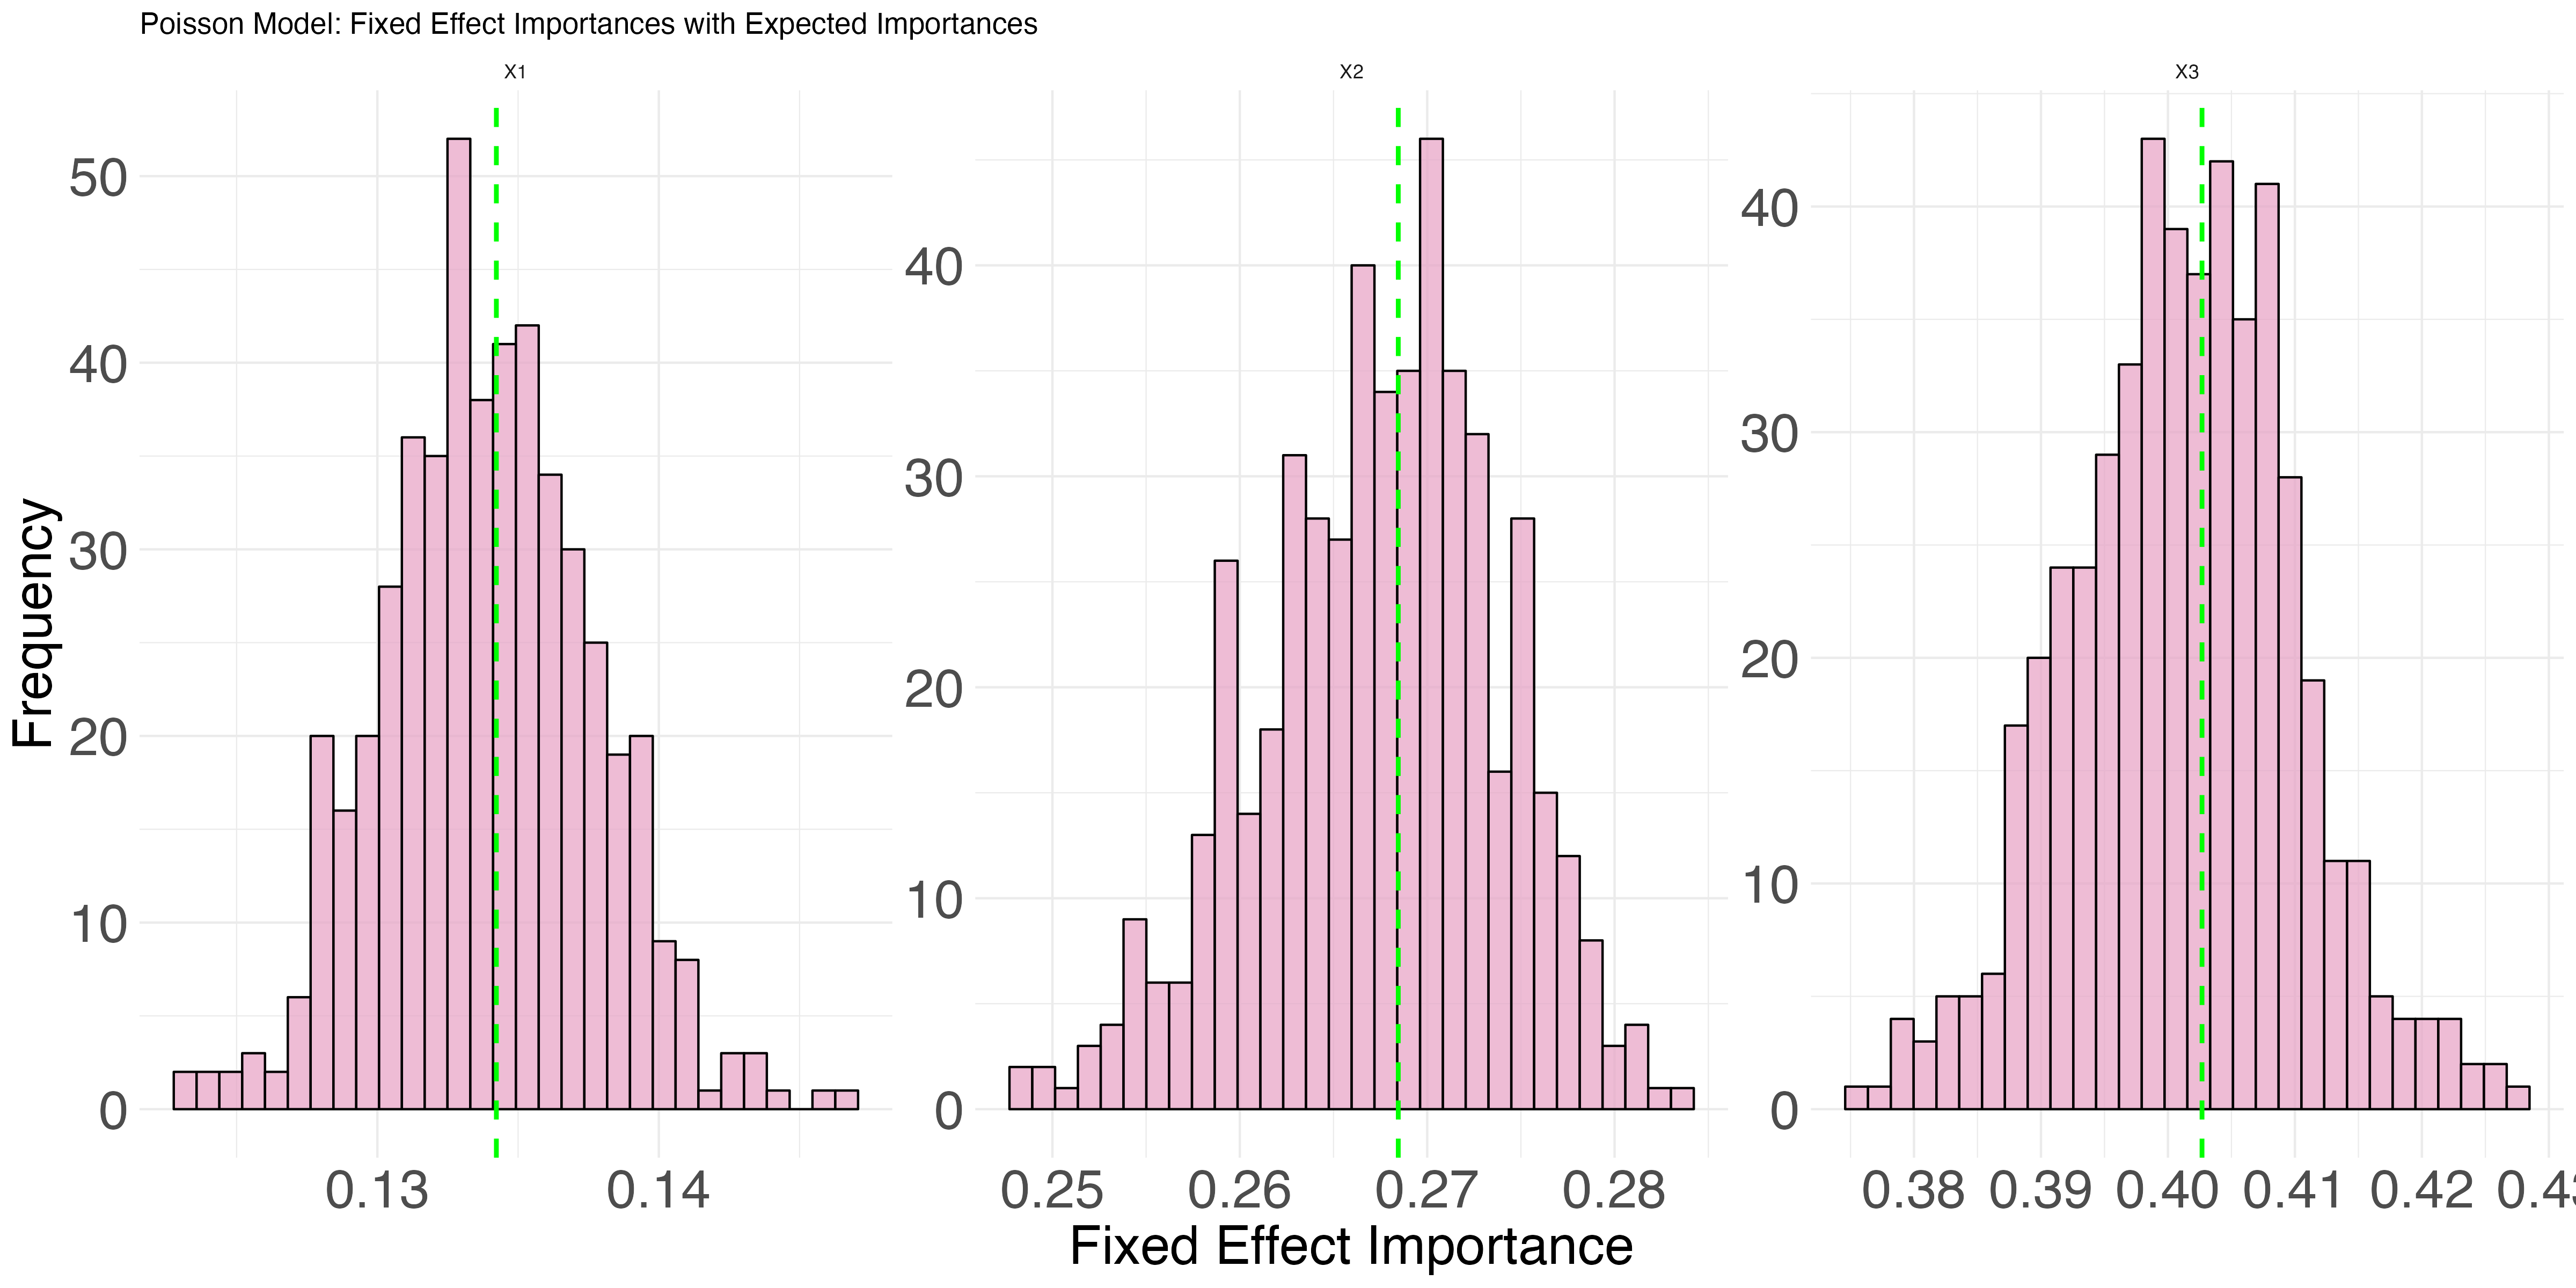
\includegraphics[width=0.7\linewidth]{Figures/Simulation study/Fixed_poisson.png}
    \caption{Relative importance of fixed effects for poisson GLMM}
    \label{fig:relimp_poisson_fixed}
\end{figure}
\begin{figure}[H]\ContinuedFloat
  \centering
  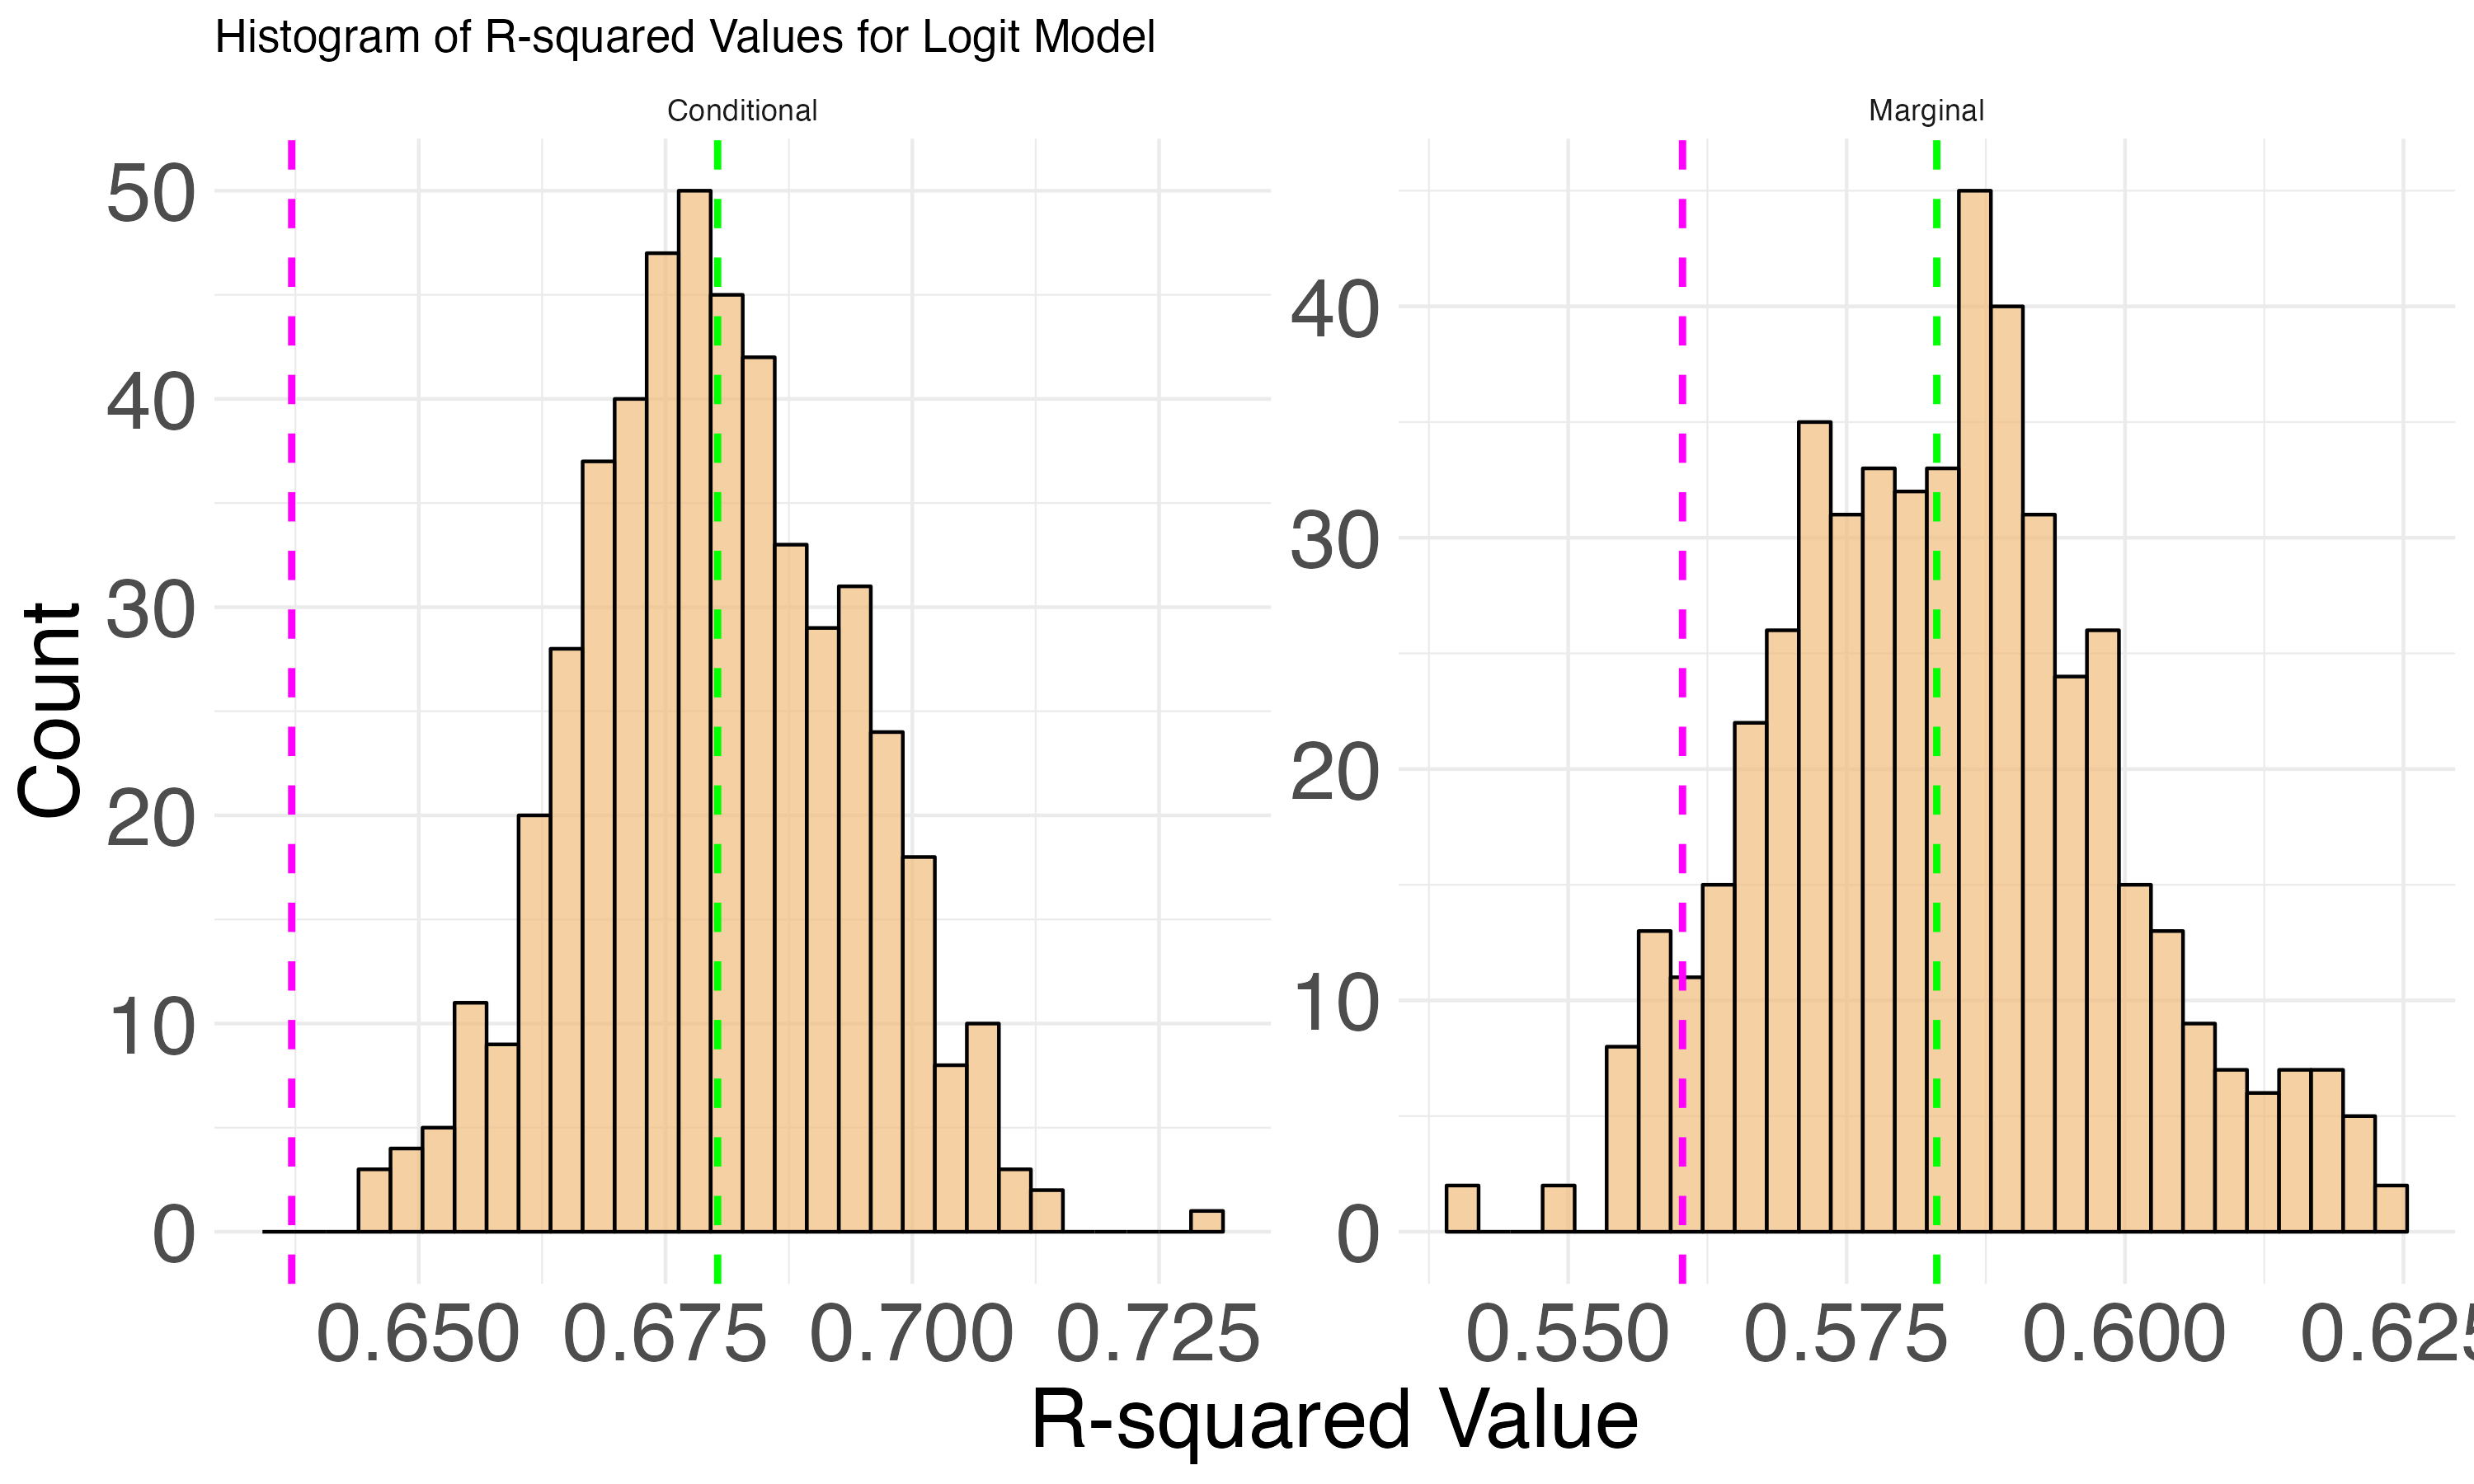
\includegraphics[width=0.7\linewidth]{Figures/Simulation study/R2_logit.png}
  \caption{Conditional and marginal $R^2$ for poisson GLMM. The magenta line is Stoffel, green line is expected importance}
    \label{fig:relimp_poisson_R2}
\end{figure}

